\documentclass[11pt]{article}
\usepackage[letterpaper,margin=1in]{geometry}
\usepackage{times}
\usepackage{latexsym}
\usepackage[T1]{fontenc}
\usepackage{booktabs}
\usepackage{array}
\usepackage{graphicx}
\usepackage{caption}
\usepackage{url}
\usepackage{float}
\usepackage{hyperref}
\usepackage{balance}
\hypersetup{
    colorlinks=true,
    linkcolor=blue,
    citecolor=blue,
    urlcolor=blue
}
\usepackage{placeins}

\setlength{\columnsep}{0.25in}
\setlength{\tabcolsep}{4pt}
\renewcommand{\arraystretch}{1.1}
\setlength{\textfloatsep}{8pt}
\setlength{\floatsep}{6pt}
\setcounter{topnumber}{3}
\setcounter{bottomnumber}{2}
\setcounter{totalnumber}{5}
\renewcommand{\topfraction}{0.85}
\renewcommand{\bottomfraction}{0.7}
\renewcommand{\textfraction}{0.1}
\setlength{\intextsep}{6pt}
\graphicspath{{output_plots/}{./}}

\title{Movie Memory Experiment: Event Segmentation and Boundary Effects on Recognition Memory}
\author{Vibe Coders}
\date{May 3, 2026}

\begin{document}
\twocolumn[
\maketitle

\begin{center}
\small
\textbf{Repository:} \href{https://github.com/Prateek-Tiwari10/BRSM_Project}{GitHub Repository}
\end{center}
\vspace{0.3cm}

\begin{abstract}
This study tests whether ending a video at a natural event boundary versus truncating it early alters recognition memory for individual frames. Participants viewed everyday activity clips and completed a forced-choice recognition task with confidence ratings. We report the data cleaning pipeline, descriptive statistics, exploratory visualizations, and nonparametric hypothesis tests for H1--H8 along with demographic checks D1--D3. Results show a reliable condition effect on accuracy, a robust boundary advantage, mixed evidence for interaction effects, and no demographic confounds.
\end{abstract}
\vspace{0.5cm}   
]

\section{Introduction}
Everyday experience unfolds as a continuous stream, yet memory is organized into discrete events. A central question in cognitive science is how and when the mind segments ongoing activity and how those boundaries influence subsequent remembering. This study examines recognition memory for frames from short video clips and asks whether memory depends on whether the clip ends at a natural event boundary or is truncated just before that boundary. This manipulation isolates boundary-related processing in memory formation.

The key premise is that boundaries are not merely perceptual markers; they reflect moments of cognitive updating. When an event ends, the system consolidates the just-completed event model while preparing a new one. If a video ends abruptly, this updating process may be interrupted, weakening memory for frames associated with the event. By contrasting intact and truncated endings, we test whether boundary processing yields a measurable advantage for later recognition.

To maintain ecological validity, the experiment uses everyday activities. Participants watch short clips and then complete a forced-choice recognition task in which they choose between a previously seen frame and a plausible lure, followed by a confidence rating. This design targets memory for specific visual details rather than narrative recall, offering a sensitive assay of boundary-related encoding.

\subsection{Theoretical Background}
\subsubsection{Event Segmentation Theory}
\textbf{Event Segmentation Theory (EST; \cite{zacks2007})}proposes that people maintain predictive models of ongoing activity. When predictions fail because the situation changes, a prediction error signals an event boundary. At that point, the current event model is updated and attention shifts to the new event. These boundary moments are therefore expected to be privileged times for encoding, as the system consolidates what just occurred and resets its predictions for what comes next.

\subsubsection{The Boundary Advantage Effect}
\textbf{The Boundary Advantage Effect (\cite{swallow2009})} refers to the reliable finding that information presented near event boundaries is remembered better than information from event middles. Boundaries are associated with a transient boost in attention and memory consolidation, which strengthens memory for nearby content. This effect appears across tasks and materials, suggesting a general mechanism by which event structure shapes what is remembered.

\subsubsection{Predictions for Video Memory}
If natural boundaries support encoding, then removing or truncating them should reduce recognition memory. We therefore predict lower overall accuracy for abruptly terminated videos than for intact videos. Moreover, the effect should be strongest for frames that occur near the boundary, because these moments are most likely to benefit from boundary-related consolidation. Frames from the middle of events should be less sensitive to boundary disruption, providing a contrast that isolates the boundary-specific component of the effect.

\section{Experimental Design and Hypotheses}
\subsection{Design Overview}
Participants were randomly assigned to one of two between-subjects conditions:
\begin{itemize}
  \item \textbf{NB (Natural Boundary) Condition}: Videos ended at natural event boundaries (e.g., a person completing an action, a scene concluding)
  \item \textbf{AB (Abrupt Boundary) Condition}: Videos were truncated 1--5 seconds before the natural boundary, creating artificial endings mid-event
\end{itemize}

All participants viewed 40 short video clips (17--57 seconds each) depicting everyday activities. After the viewing phase, participants completed a forced-choice recognition task for 40 trials. Each trial presented two video frames: one frame actually shown in the video (target) and one similar frame not shown (lure). Participants selected which frame they had seen and rated their confidence (1--5 scale).

\subsection{Frame Types}
Each recognition trial tested one of two frame types:
\begin{itemize}
  \item \textbf{BB (Before Boundary)}: Frames from 0--3 seconds before the natural event boundary
  \item \textbf{EM (Event Middle)}: Frames from the middle of the event, far from boundaries
\end{itemize}

This within-subjects manipulation allowed us to test whether boundary effects are specific to boundary-adjacent frames or generalize across the entire event.

\subsection{Study Hypotheses}
\textbf{Hypothesis 1 (Main Effect):} NB participants will demonstrate higher overall recognition accuracy than AB participants. Rationale: Natural boundaries allow complete event model updating and memory consolidation, while abrupt truncation interrupts this process.

\textbf{Hypothesis 2 (Boundary Frame Advantage):} The NB advantage will be significantly stronger for BB frames than for EM frames. Rationale: BB frames are most proximal to the disrupted boundary and should be most affected by boundary presence or absence.

\textbf{Hypothesis 3 (Null Effect on EM Frames):} NB and AB conditions will not differ significantly on EM frame accuracy. Rationale: Frames from event middles are temporally distant from the disrupted boundary and should be minimally affected by the manipulation.

\section{Data and Data Cleaning}
\subsection{Data Structure and Cleaning Pipeline}
The behavioral dataset initially consisted of 165 participants and approximately 6,600 trials prior to preprocessing. A structured data cleaning pipeline was applied to ensure data integrity, consistency, and reliability of subsequent analyses.

First, demographic records were validated and aligned with individual participant CSV files using unique participant identifiers. Condition labels (NB vs.\ AB) were cross-verified and synchronized using filename-based ground truth to eliminate any potential mismatches.

Next, response-time (RT) based filtering was performed to remove implausible or noisy observations. Trials with extremely fast responses (RT $< 200$ ms) were excluded, as such responses are unlikely to reflect genuine cognitive processing and may instead indicate accidental or anticipatory key presses. Additionally, trials with excessively long response times (RT $>$ mean $+ 3 \times$ SD) were removed to mitigate the influence of outliers and lapses in attention.

At the participant level, individuals with unusually long total encoding durations were excluded based on a predefined cutoff, ensuring that extreme behavioral patterns did not bias the results.

These preprocessing steps resulted in a cleaned dataset that balances robustness and data retention, preserving meaningful variability while removing noise. The tables below summarize the key cleaning steps, exclusion criteria, and the final post-exclusion dataset used for all analyses.
\begin{table}[htbp]
\centering
\small
\caption{Demographic data validation and imputation summary}
\makebox[\columnwidth][c]{\begin{tabular}{lr}
\toprule
Metric & Value \\
\midrule
Rows loaded & 185 \\
Rows after participant\_id validation & 185 \\
Rows removed for missing/empty participant\_id & 0 \\
Missing Age after imputation & 0 \\
Missing Gender after imputation & 0 \\
Missing Handedness after imputation & 0 \\
Missing Vision after imputation & 0 \\
\bottomrule
\end{tabular}}
\end{table}

\begin{table}[htbp]
\centering
\small
\caption{Exclusion and flagging summary}
\makebox[\columnwidth][c]{\begin{tabular}{lr}
\toprule
Criterion & Count \\
\midrule
Participants excluded: encoding time $>$ 27.05 minutes & 5 \\
Trials flagged: RT $<$ 0.2 s & 0 \\
Trials flagged: RT $>$ mean + 3 SD & 122 \\
\bottomrule
\end{tabular}}
\end{table}

\begin{table}[htbp]
\centering
\small
\caption{Post-exclusion data snapshot}
\makebox[\columnwidth][c]{\begin{tabular}{lr}
\toprule
Metric & Value \\
\midrule
Original trial rows & 6800 \\
Trial rows after all exclusions & 6487 \\
Unique participants after exclusion & 165 \\
Min RT after exclusion (s) & 0.276 \\
Max RT after exclusion (s) & 17.1 \\
Mean RT after exclusion (s) & 5.37 \\
\bottomrule
\end{tabular}}
\end{table}

\section{Variables and Descriptive Analysis}
\subsection{Variable Types}
IVs: Condition (between-subjects, nominal: NB/AB); FrameType (within-subjects, nominal: BB/EM). DVs: Accuracy (ratio: 0--1), RT (ratio: seconds), Confidence (ordinal: 1--5). Demographics: Age (ratio: years), Gender (nominal), Handedness (nominal), Vision (nominal).

\subsection{Sample Characteristics}
Final analytic sample size: N = 165 participants (after exclusions). Condition assignment: NB N = 87, AB N = 78. The randomization produced reasonably balanced groups for subsequent independent-samples comparisons.

\subsection{Demographic Summary Statistics}
\begin{table}[htbp]
\centering
\small
\caption{Participant demographics (complete records)}
\makebox[\columnwidth][c]{\begin{tabular}{lr}
\toprule
Characteristic & Value \\
\midrule
N (complete demographic records) & 185 \\
Age - Mean (SD) & 22.3 (2.2) \\
Age - Range & 19--34 \\
Female & 50 \\
Male & 135 \\
Right-handed & 176 \\
Left-handed & 9 \\
Normal vision & 106 \\
Corrected to normal & 77 \\
Uncorrected vision difficulty & 2 \\
\bottomrule
\end{tabular}}
\end{table}

\begin{table}[htbp]
\centering
\small
\caption{Demographics by condition}
\makebox[\columnwidth][c]{\begin{tabular}{lrrrr}
\toprule
Condition & N & Age M & Age SD & Female \\
\midrule
AB & 91 & 22.3 & 2.1 & 27 \\
NB & 94 & 22.2 & 2.2 & 23 \\
\bottomrule
\end{tabular}}
\end{table}


\begin{table}[H]
\centering
\small
\caption{Overall accuracy by condition}
\makebox[\columnwidth][c]{\begin{tabular}{lrrrrrr}
\toprule
Condition & N & Mean & SD & SE & Min & Max \\
\midrule
NB & 87 & 0.876 & 0.072 & 0.008 & 0.650 & 1.000 \\
AB & 78 & 0.843 & 0.082 & 0.009 & 0.575 & 1.000 \\
\bottomrule
\end{tabular}}
\end{table}

\begin{table}[!t]
\centering
\small
\caption{Accuracy by condition and frame type}
\makebox[\columnwidth][c]{\begin{tabular}{lrrrrr}
\toprule
Condition & FrameType & N & Mean & SD \\
\midrule
NB & BB & 87 & 0.863 & 0.095 \\
NB & EM & 87 & 0.890 & 0.079 \\
AB & BB & 78 & 0.826 & 0.107 \\
AB & EM & 78 & 0.860 & 0.091 \\
\bottomrule
\end{tabular}}
\end{table}

\begin{table}[!t]
\centering
\small
\caption{Reaction time and confidence by condition}
\makebox[\columnwidth][c]{\begin{tabular}{lrrrrr}
\toprule
Condition & Trials & Mean RT & SD RT & Mean Conf & SD Conf \\
\midrule
NB & 3415 & 5.43 & 2.80 & 4.23 & 1.08 \\
AB & 3072 & 5.31 & 2.83 & 4.09 & 1.17 \\
\bottomrule
\end{tabular}}
\end{table}

\FloatBarrier

\section{Exploratory Data Analysis}
\noindent\textbf{Note:} This section was done and submitted in the mid-sem report.

\begin{figure}[htbp]
\centering
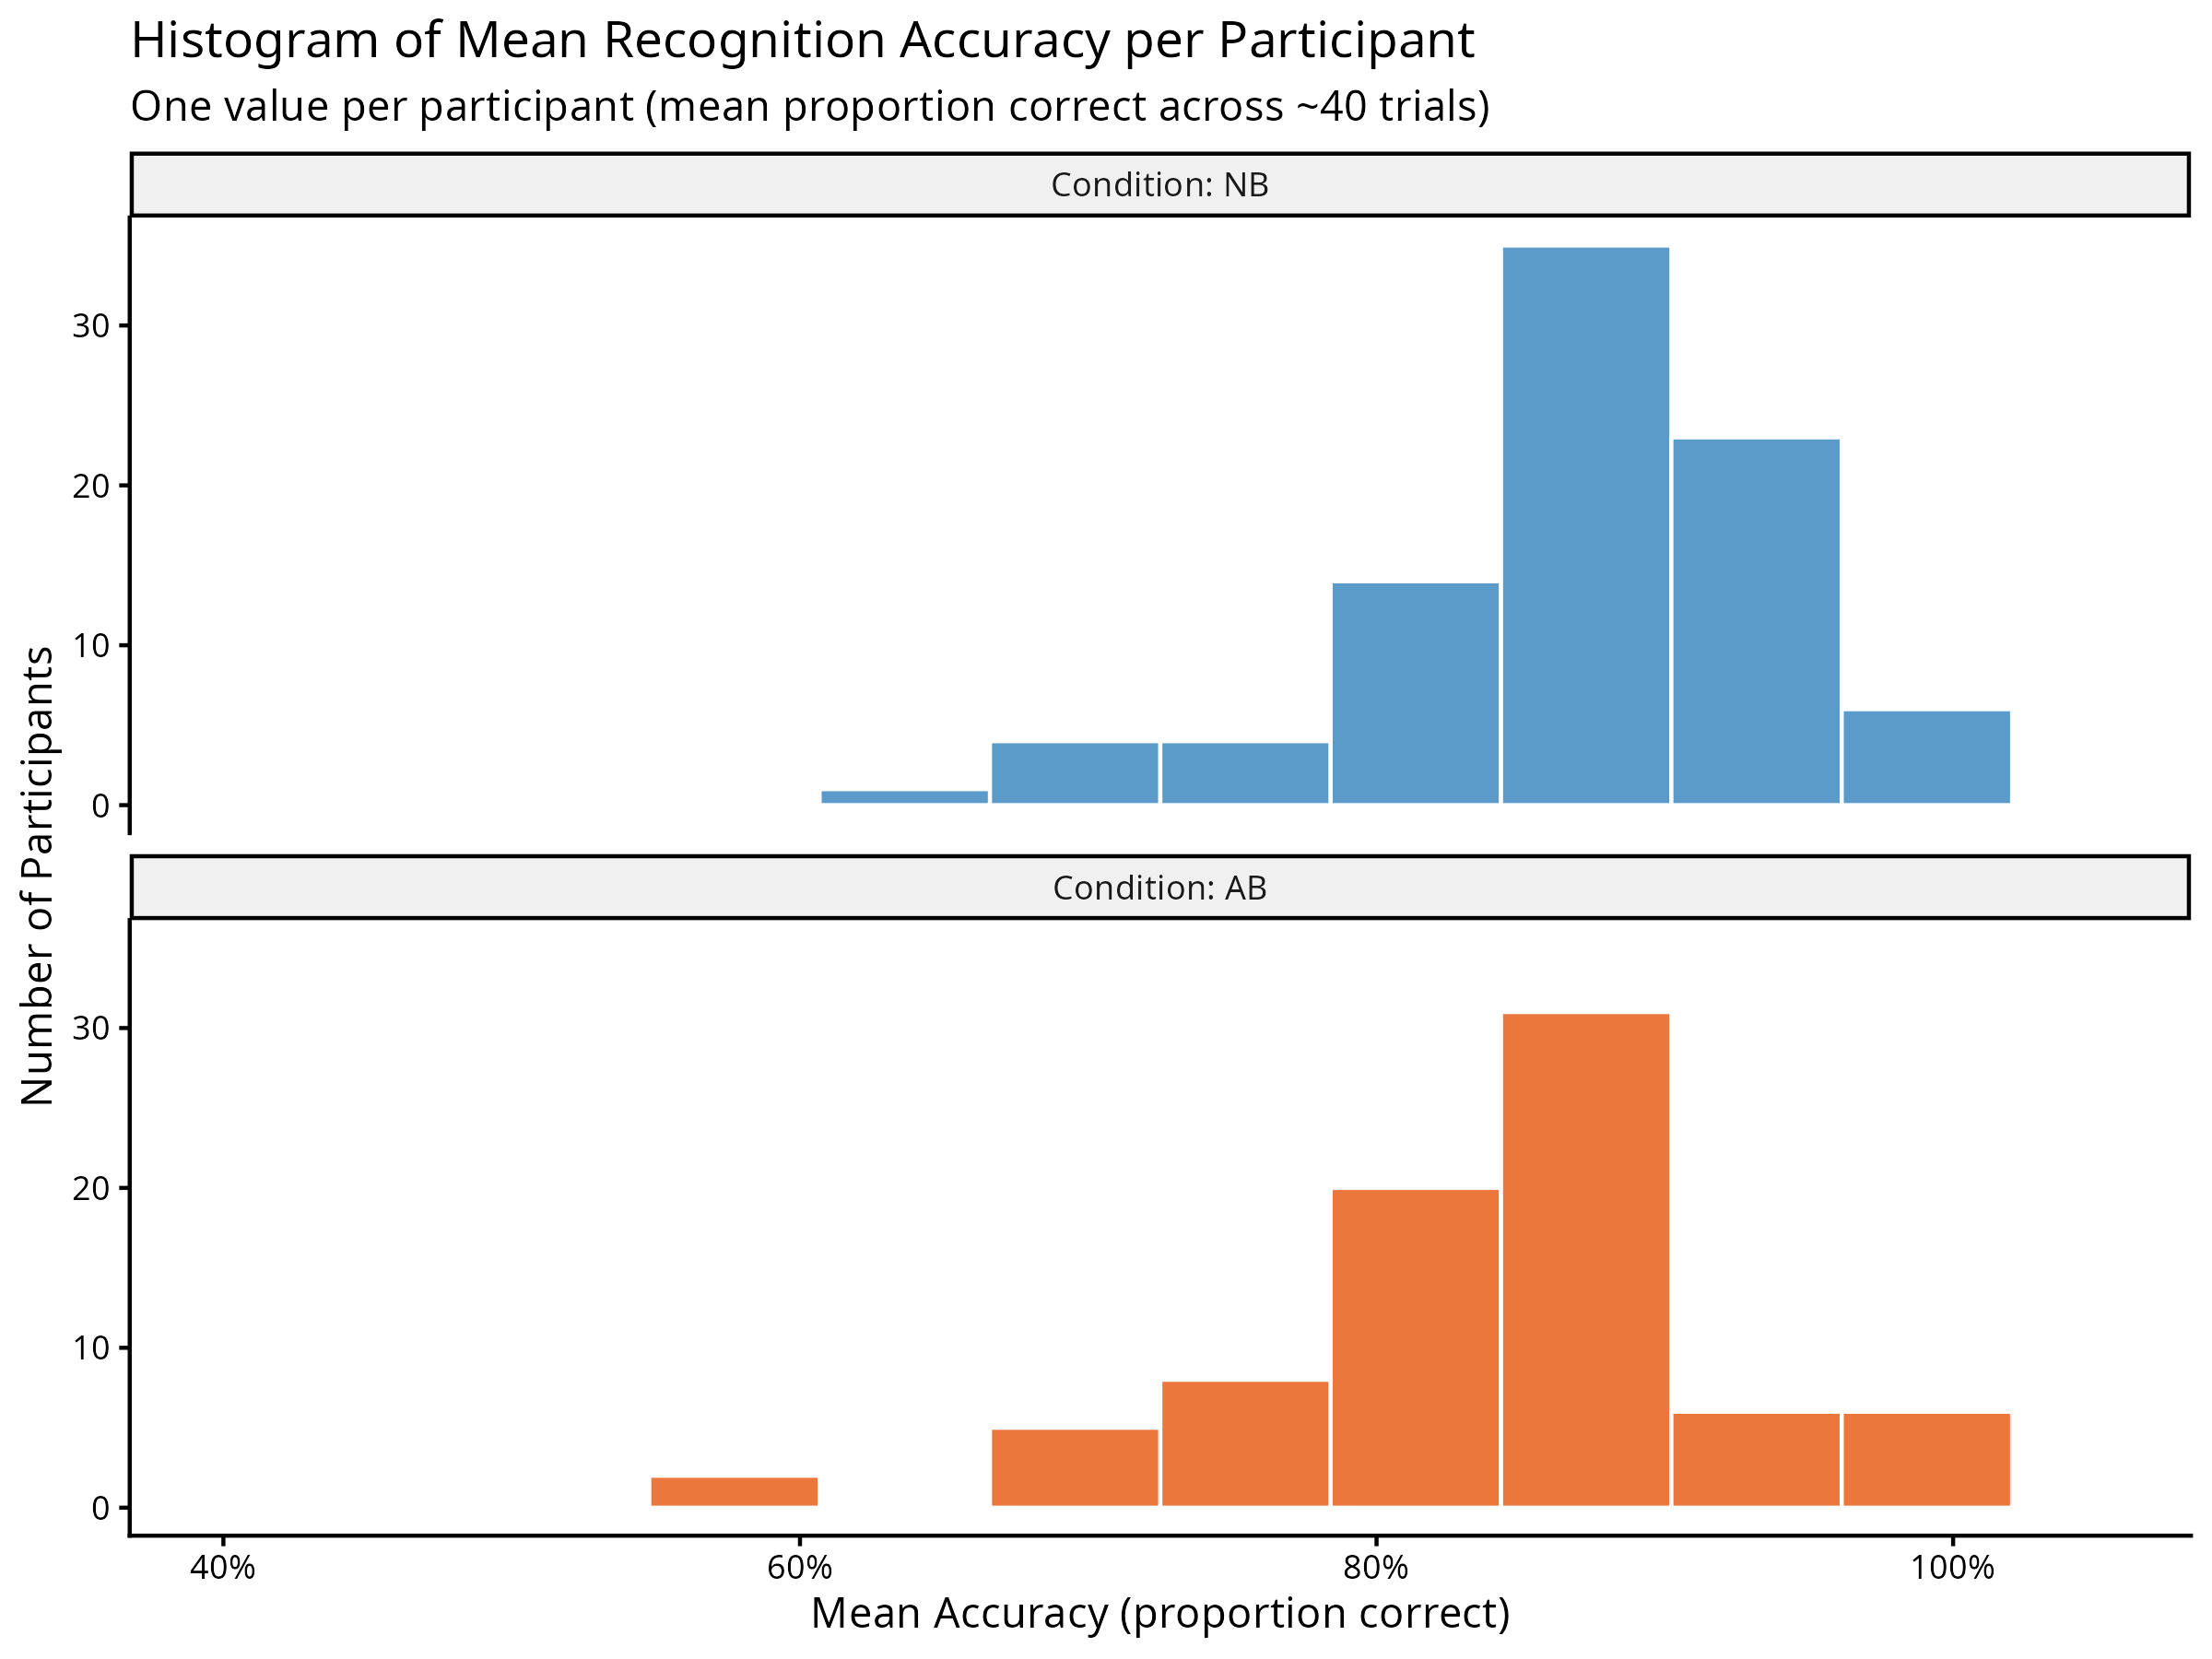
\includegraphics[width=\columnwidth]{output_plots/accuracy_histogram.png}
\caption{Histogram of mean recognition accuracy by condition.}
\end{figure}

\begin{figure}[htbp]
\centering
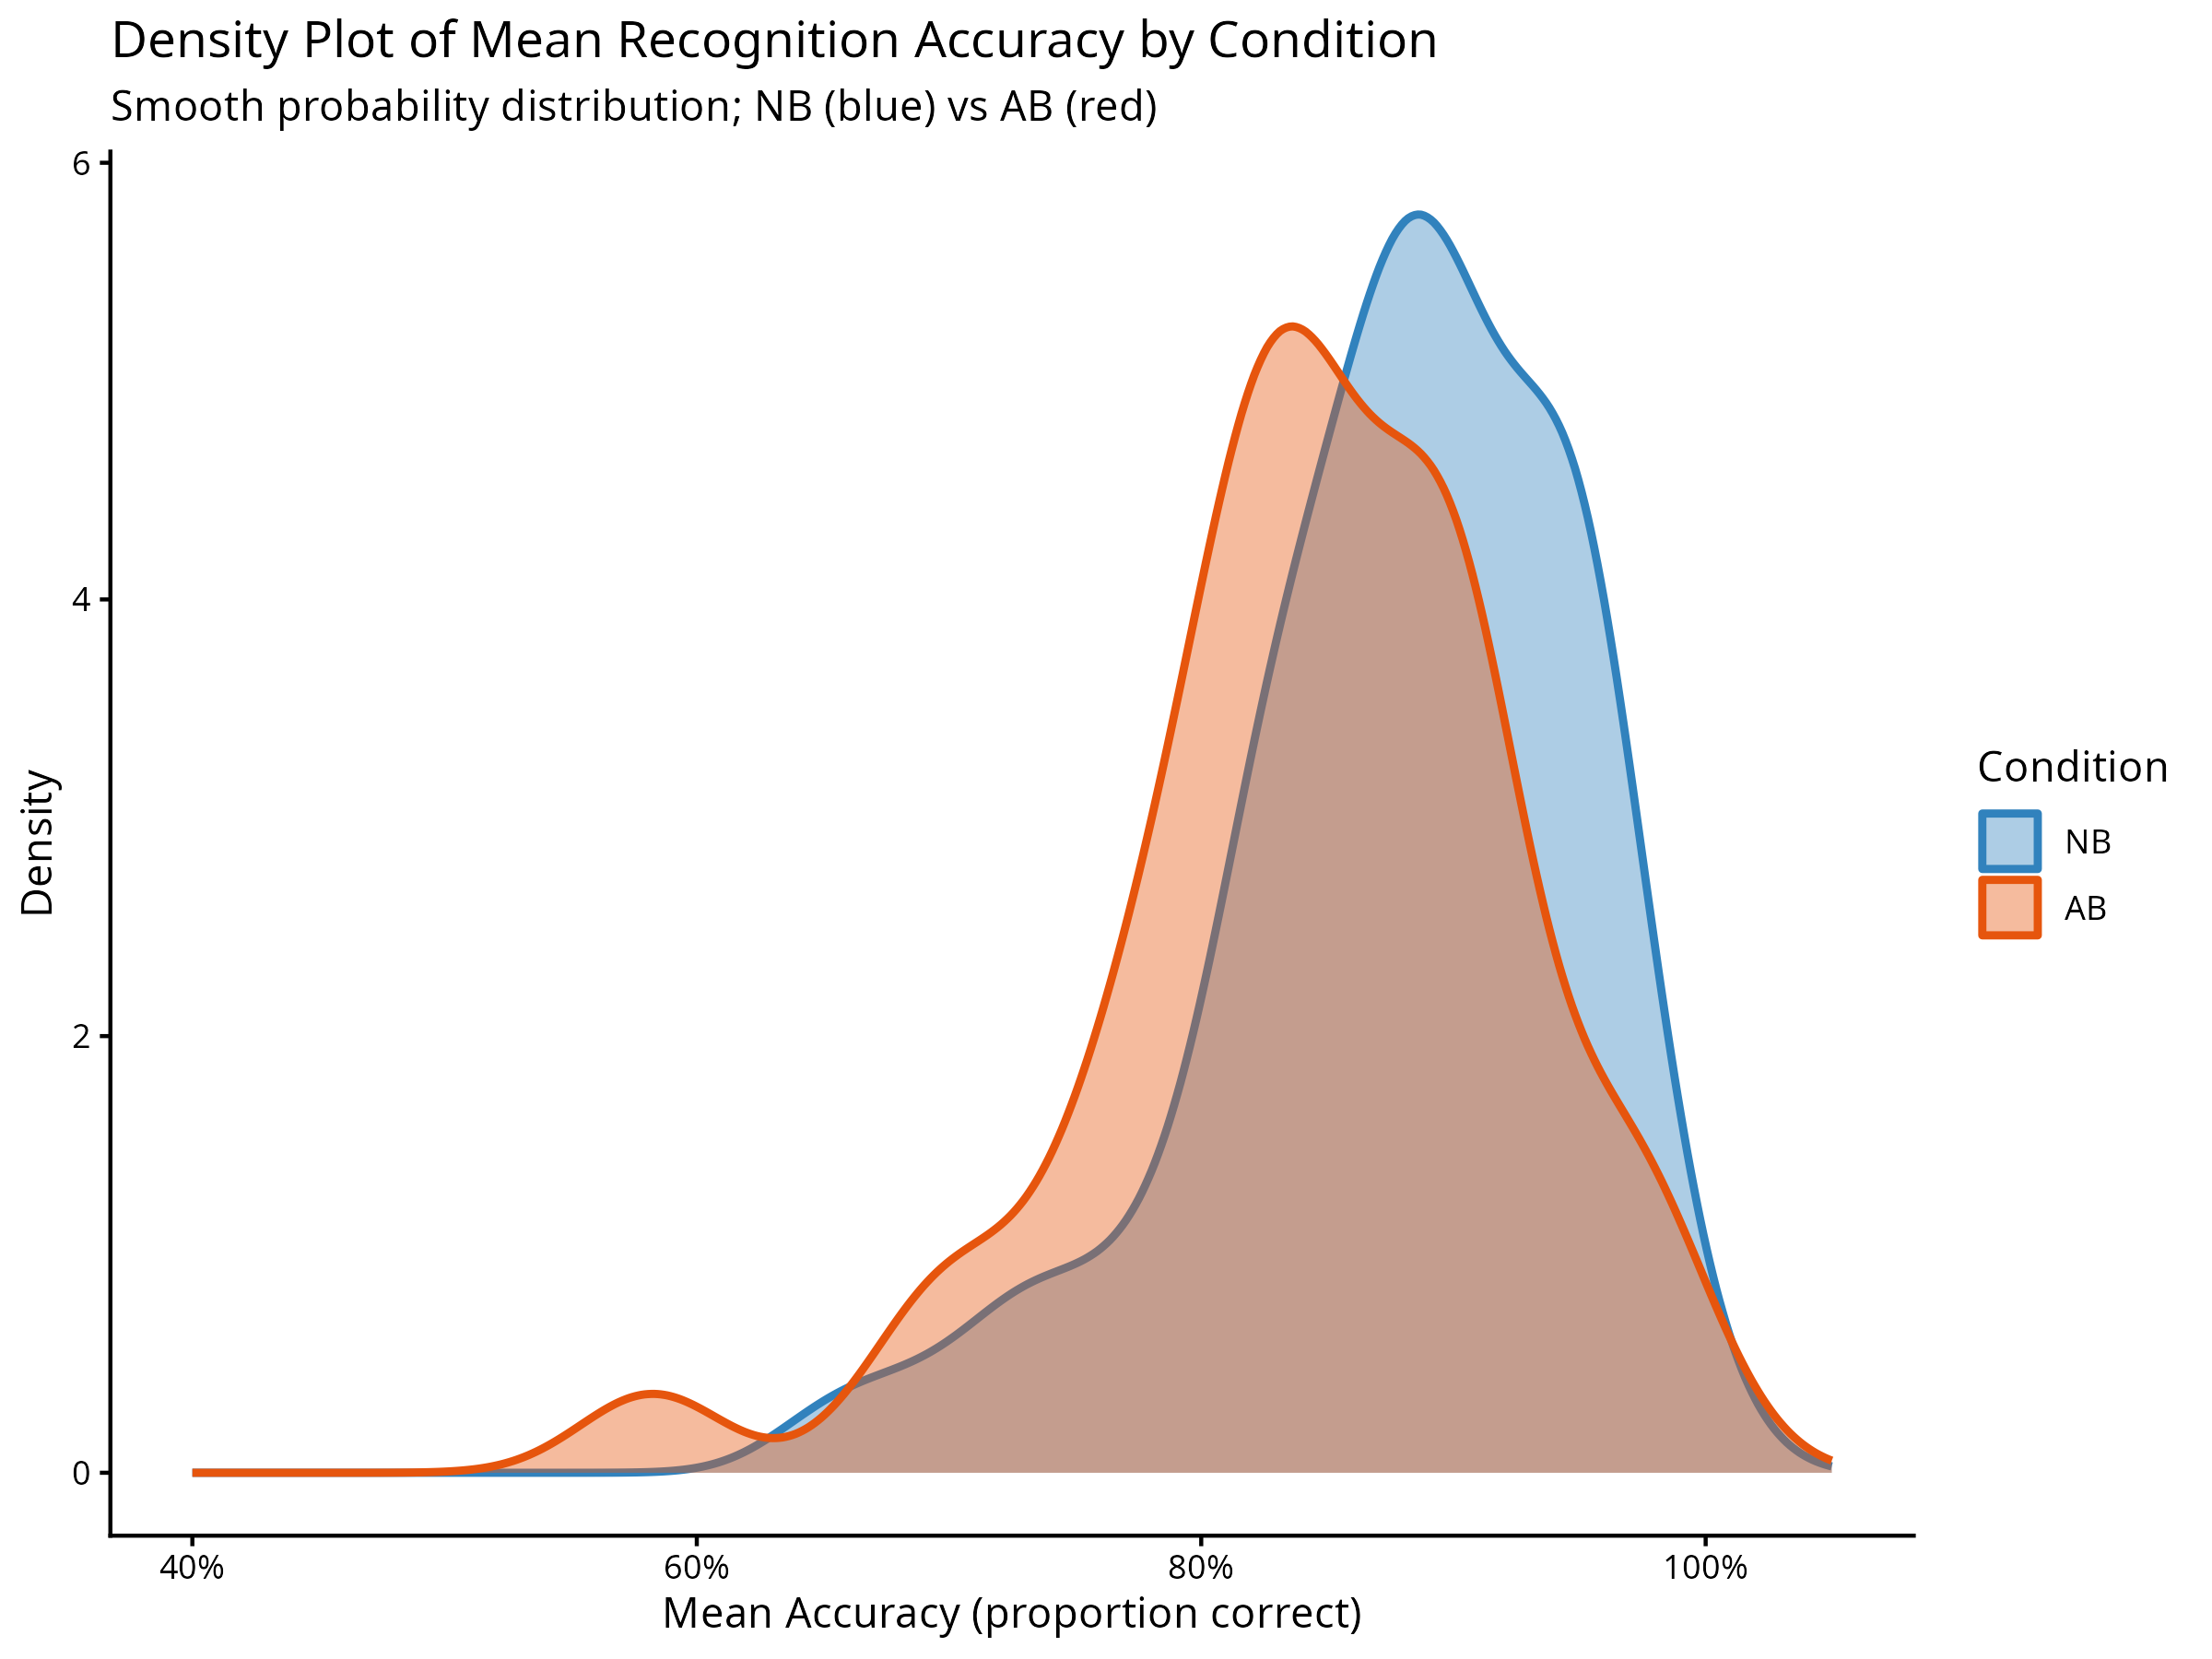
\includegraphics[width=\columnwidth]{output_plots/accuracy_density.png}
\caption{Density plot of mean recognition accuracy by condition.}
\end{figure}


\begin{figure}[htbp]
\centering
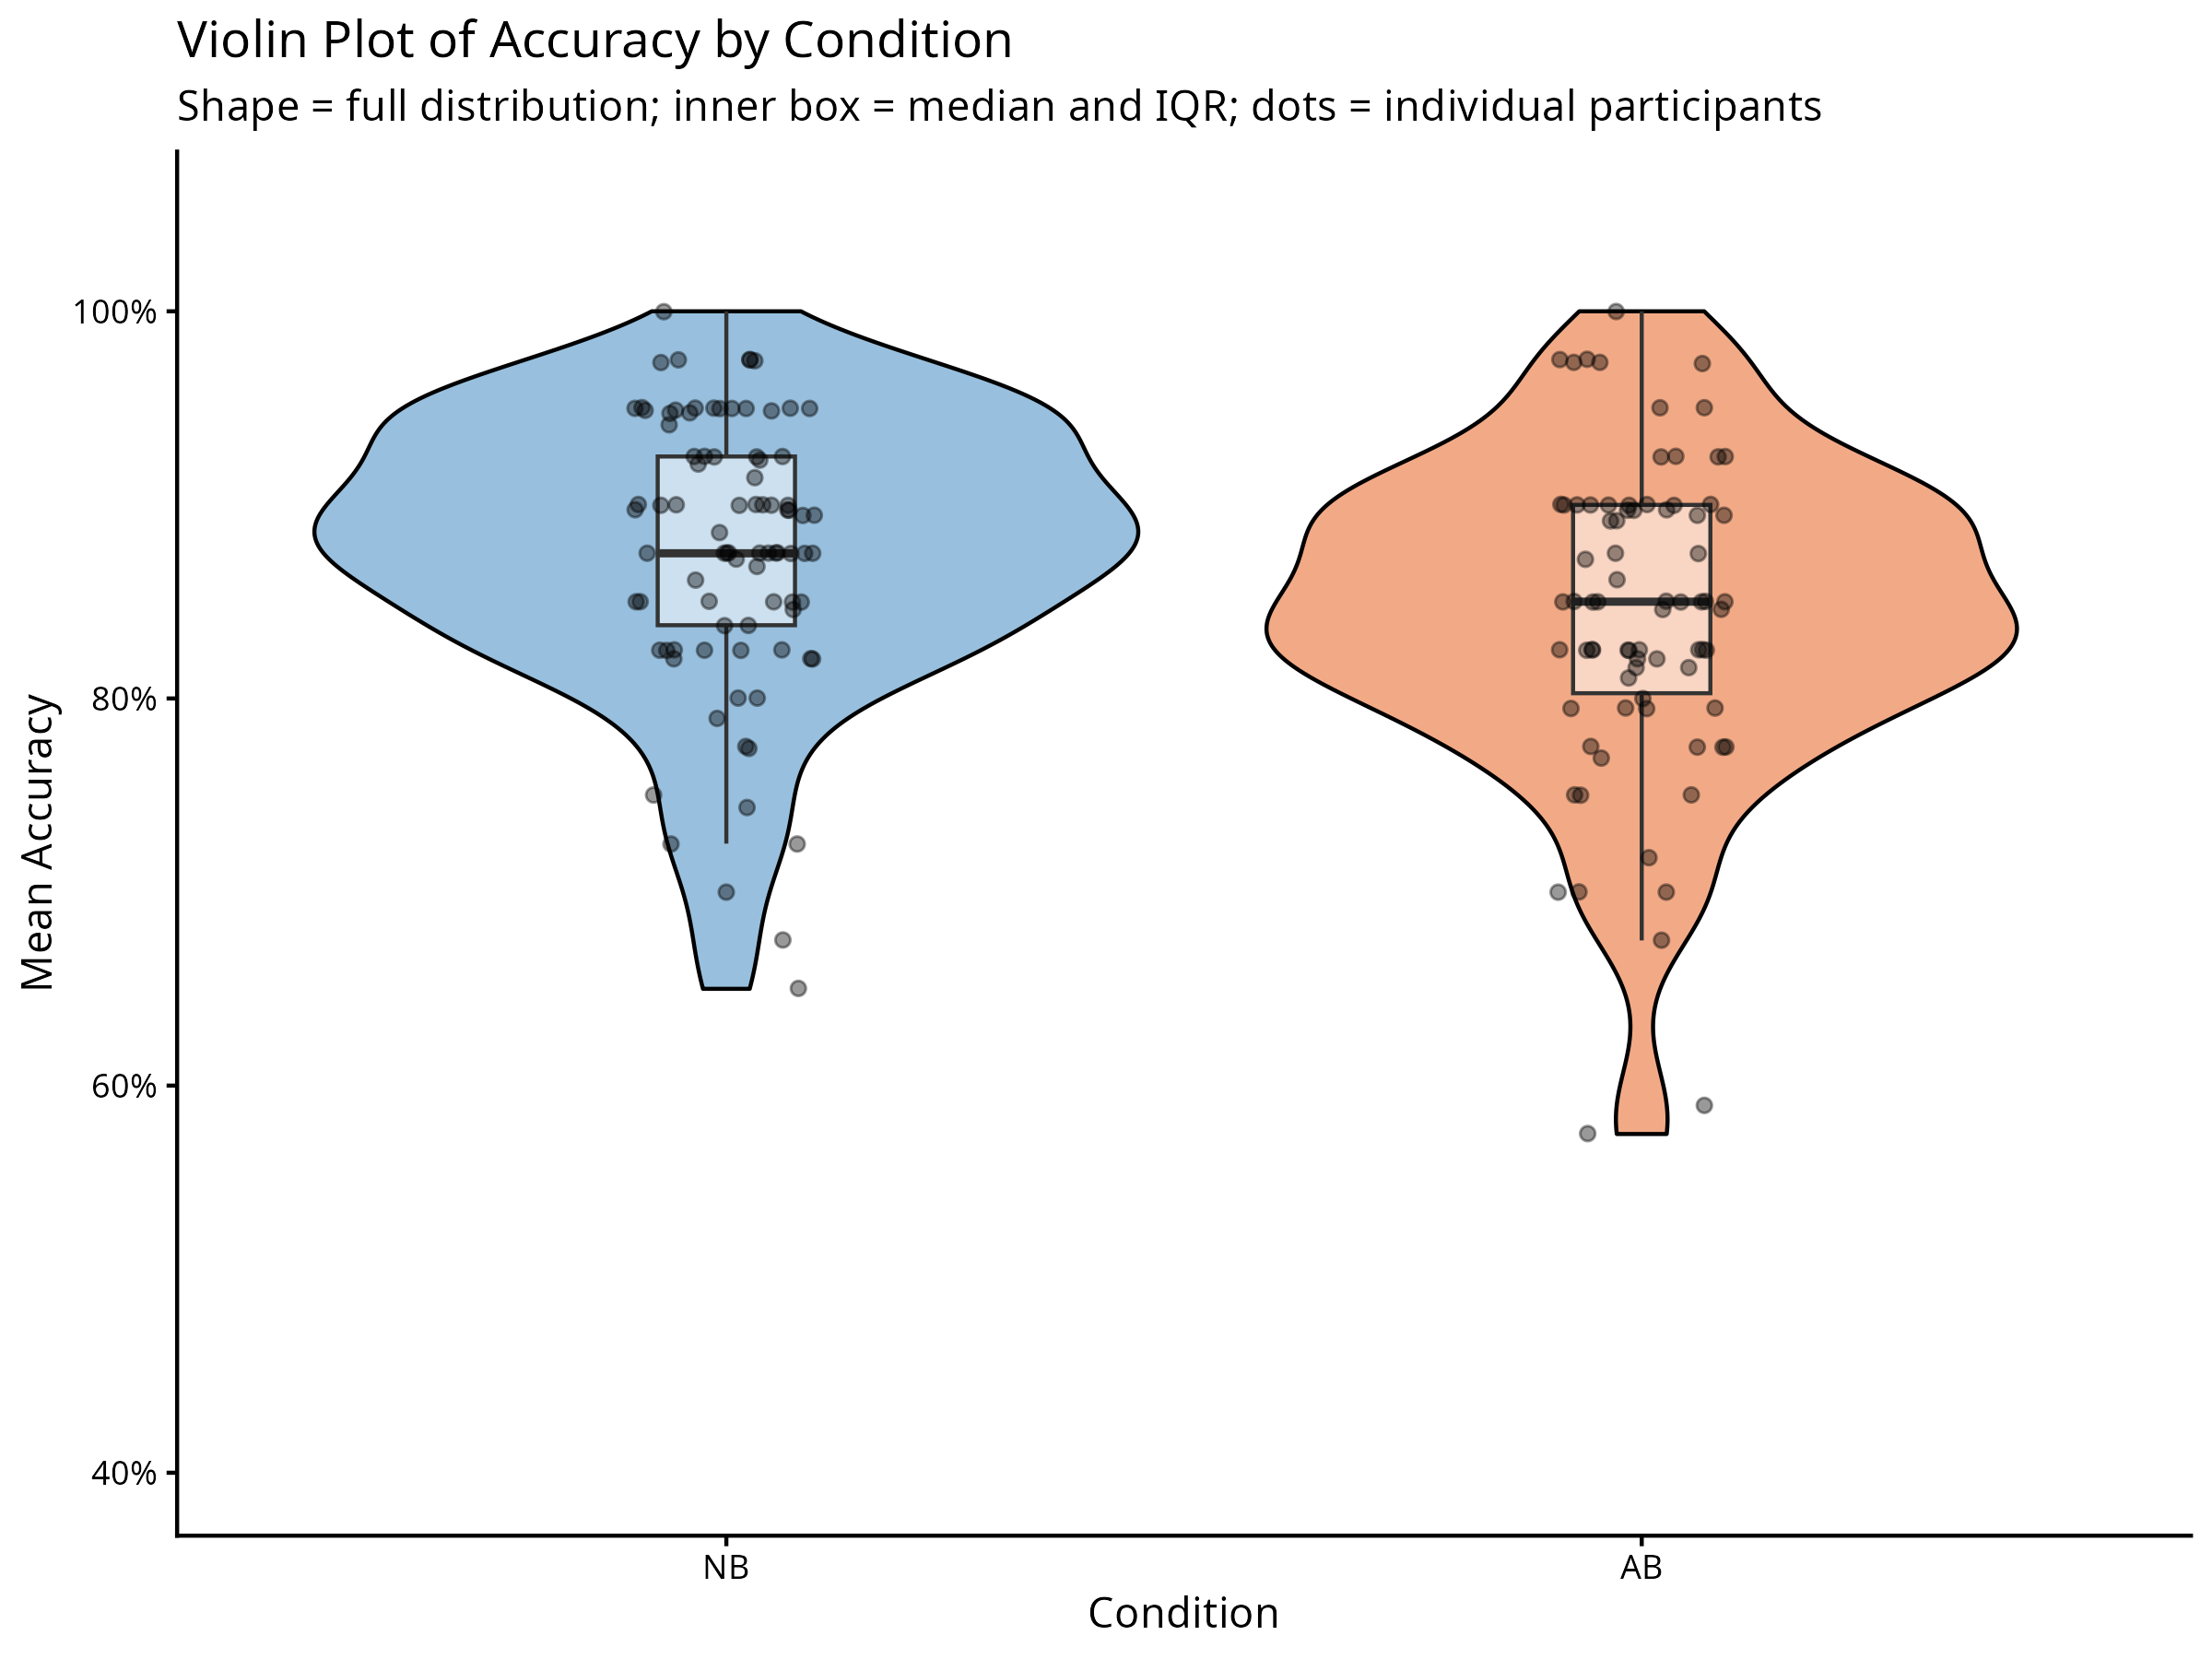
\includegraphics[width=\columnwidth]{output_plots/accuracy_condition_violin.png}
\caption{Accuracy by condition (violin plot).}
\end{figure}

\begin{figure}[htbp]
\centering
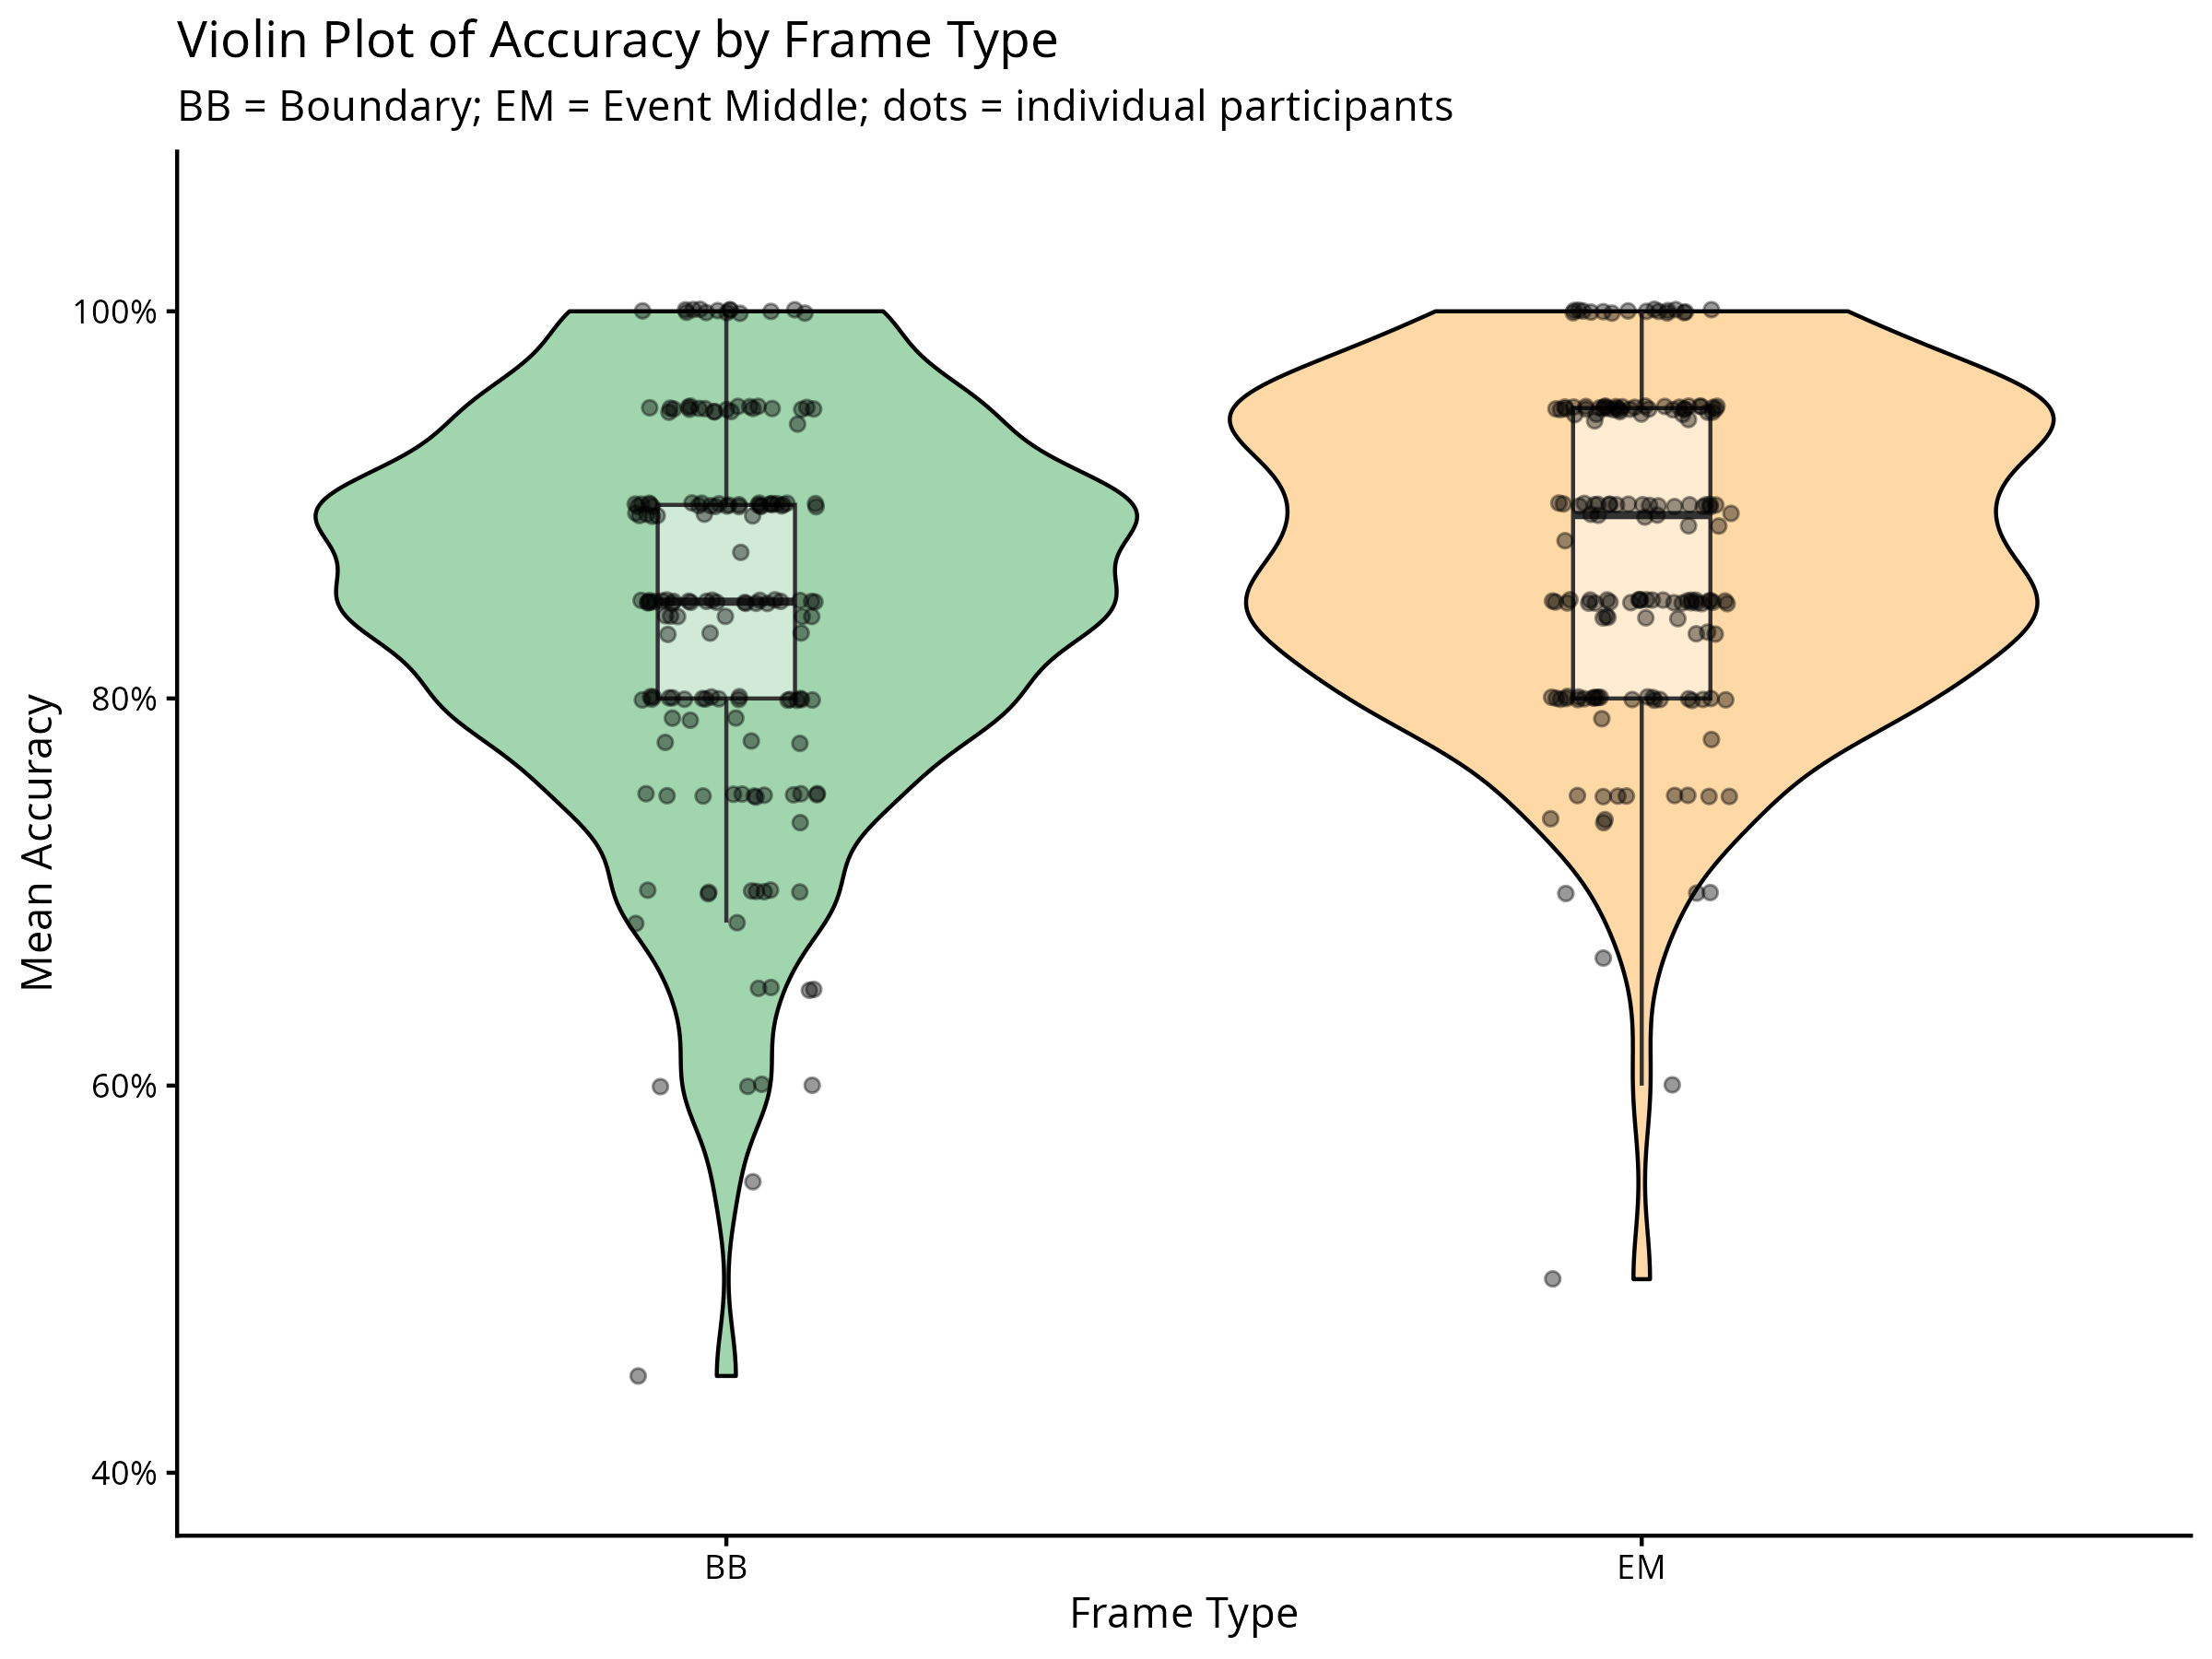
\includegraphics[width=\columnwidth]{output_plots/accuracy_frametype_violin.png}
\caption{Accuracy by frame type (violin plot).}
\end{figure}

\begin{figure}[htbp]
\centering
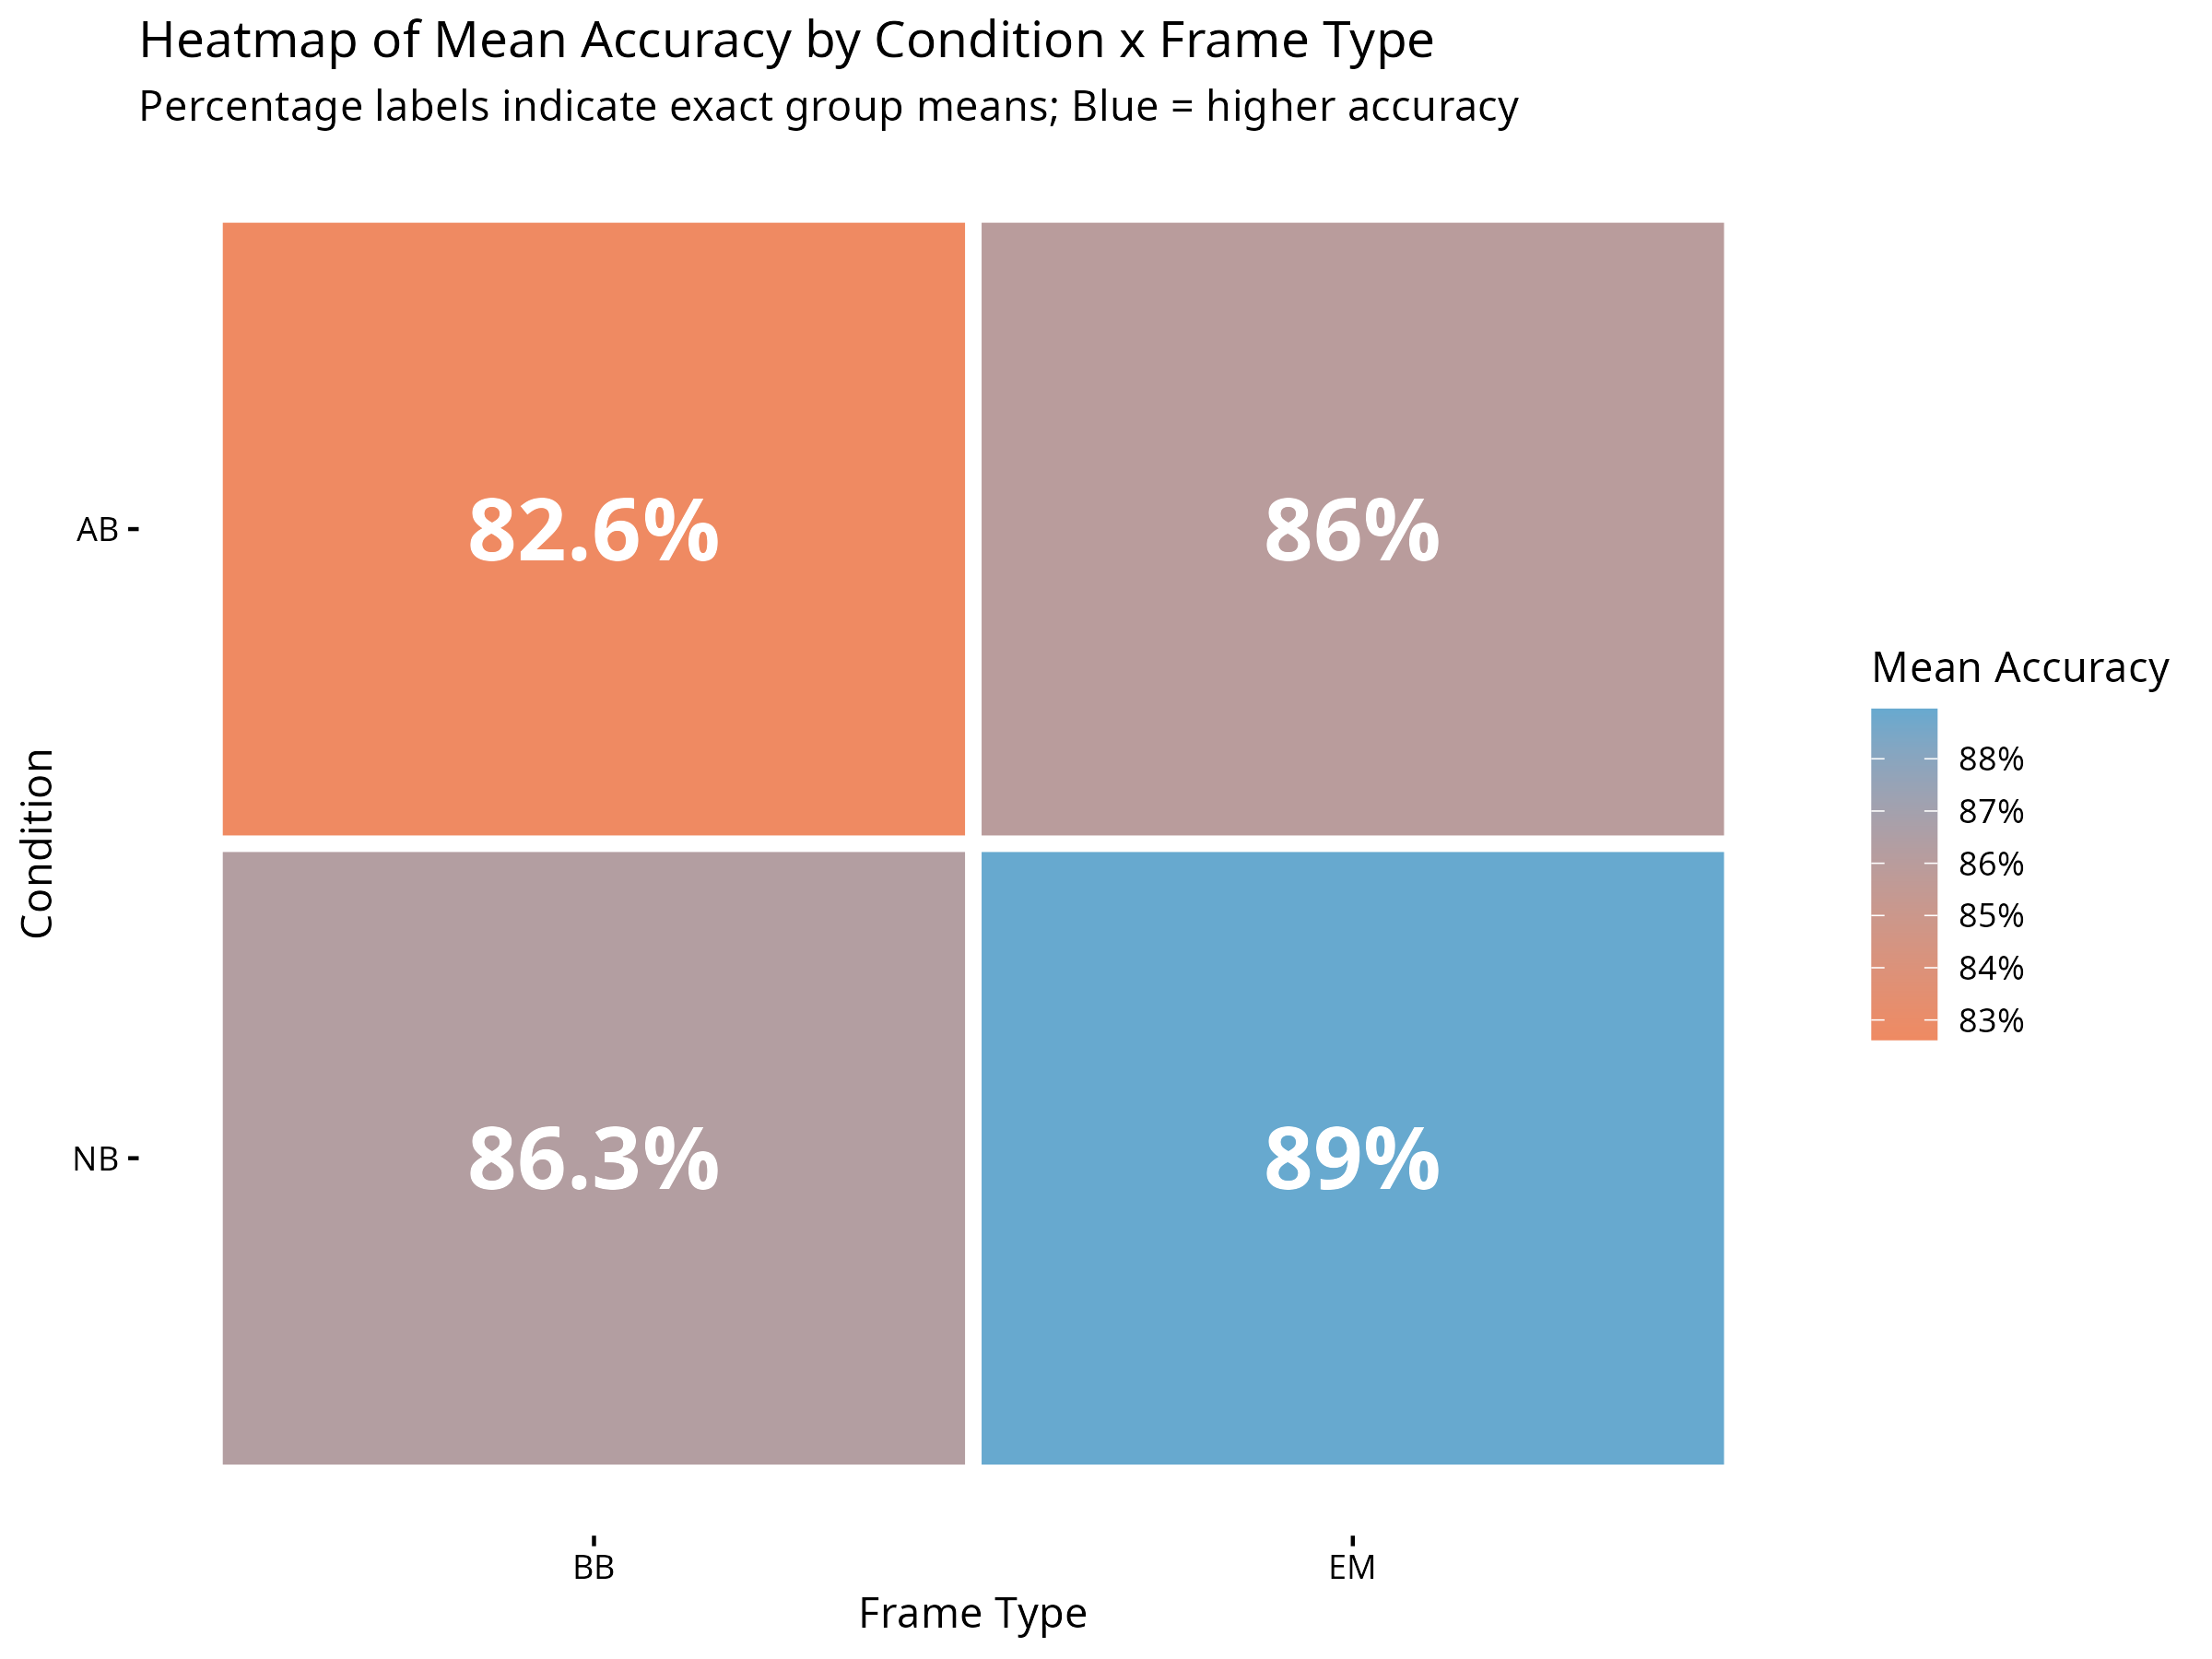
\includegraphics[width=\columnwidth]{output_plots/accuracy_interaction_heatmap.png}
\caption{Mean accuracy heatmap by Condition x FrameType.}
\end{figure}

\begin{figure}[htbp]
\centering
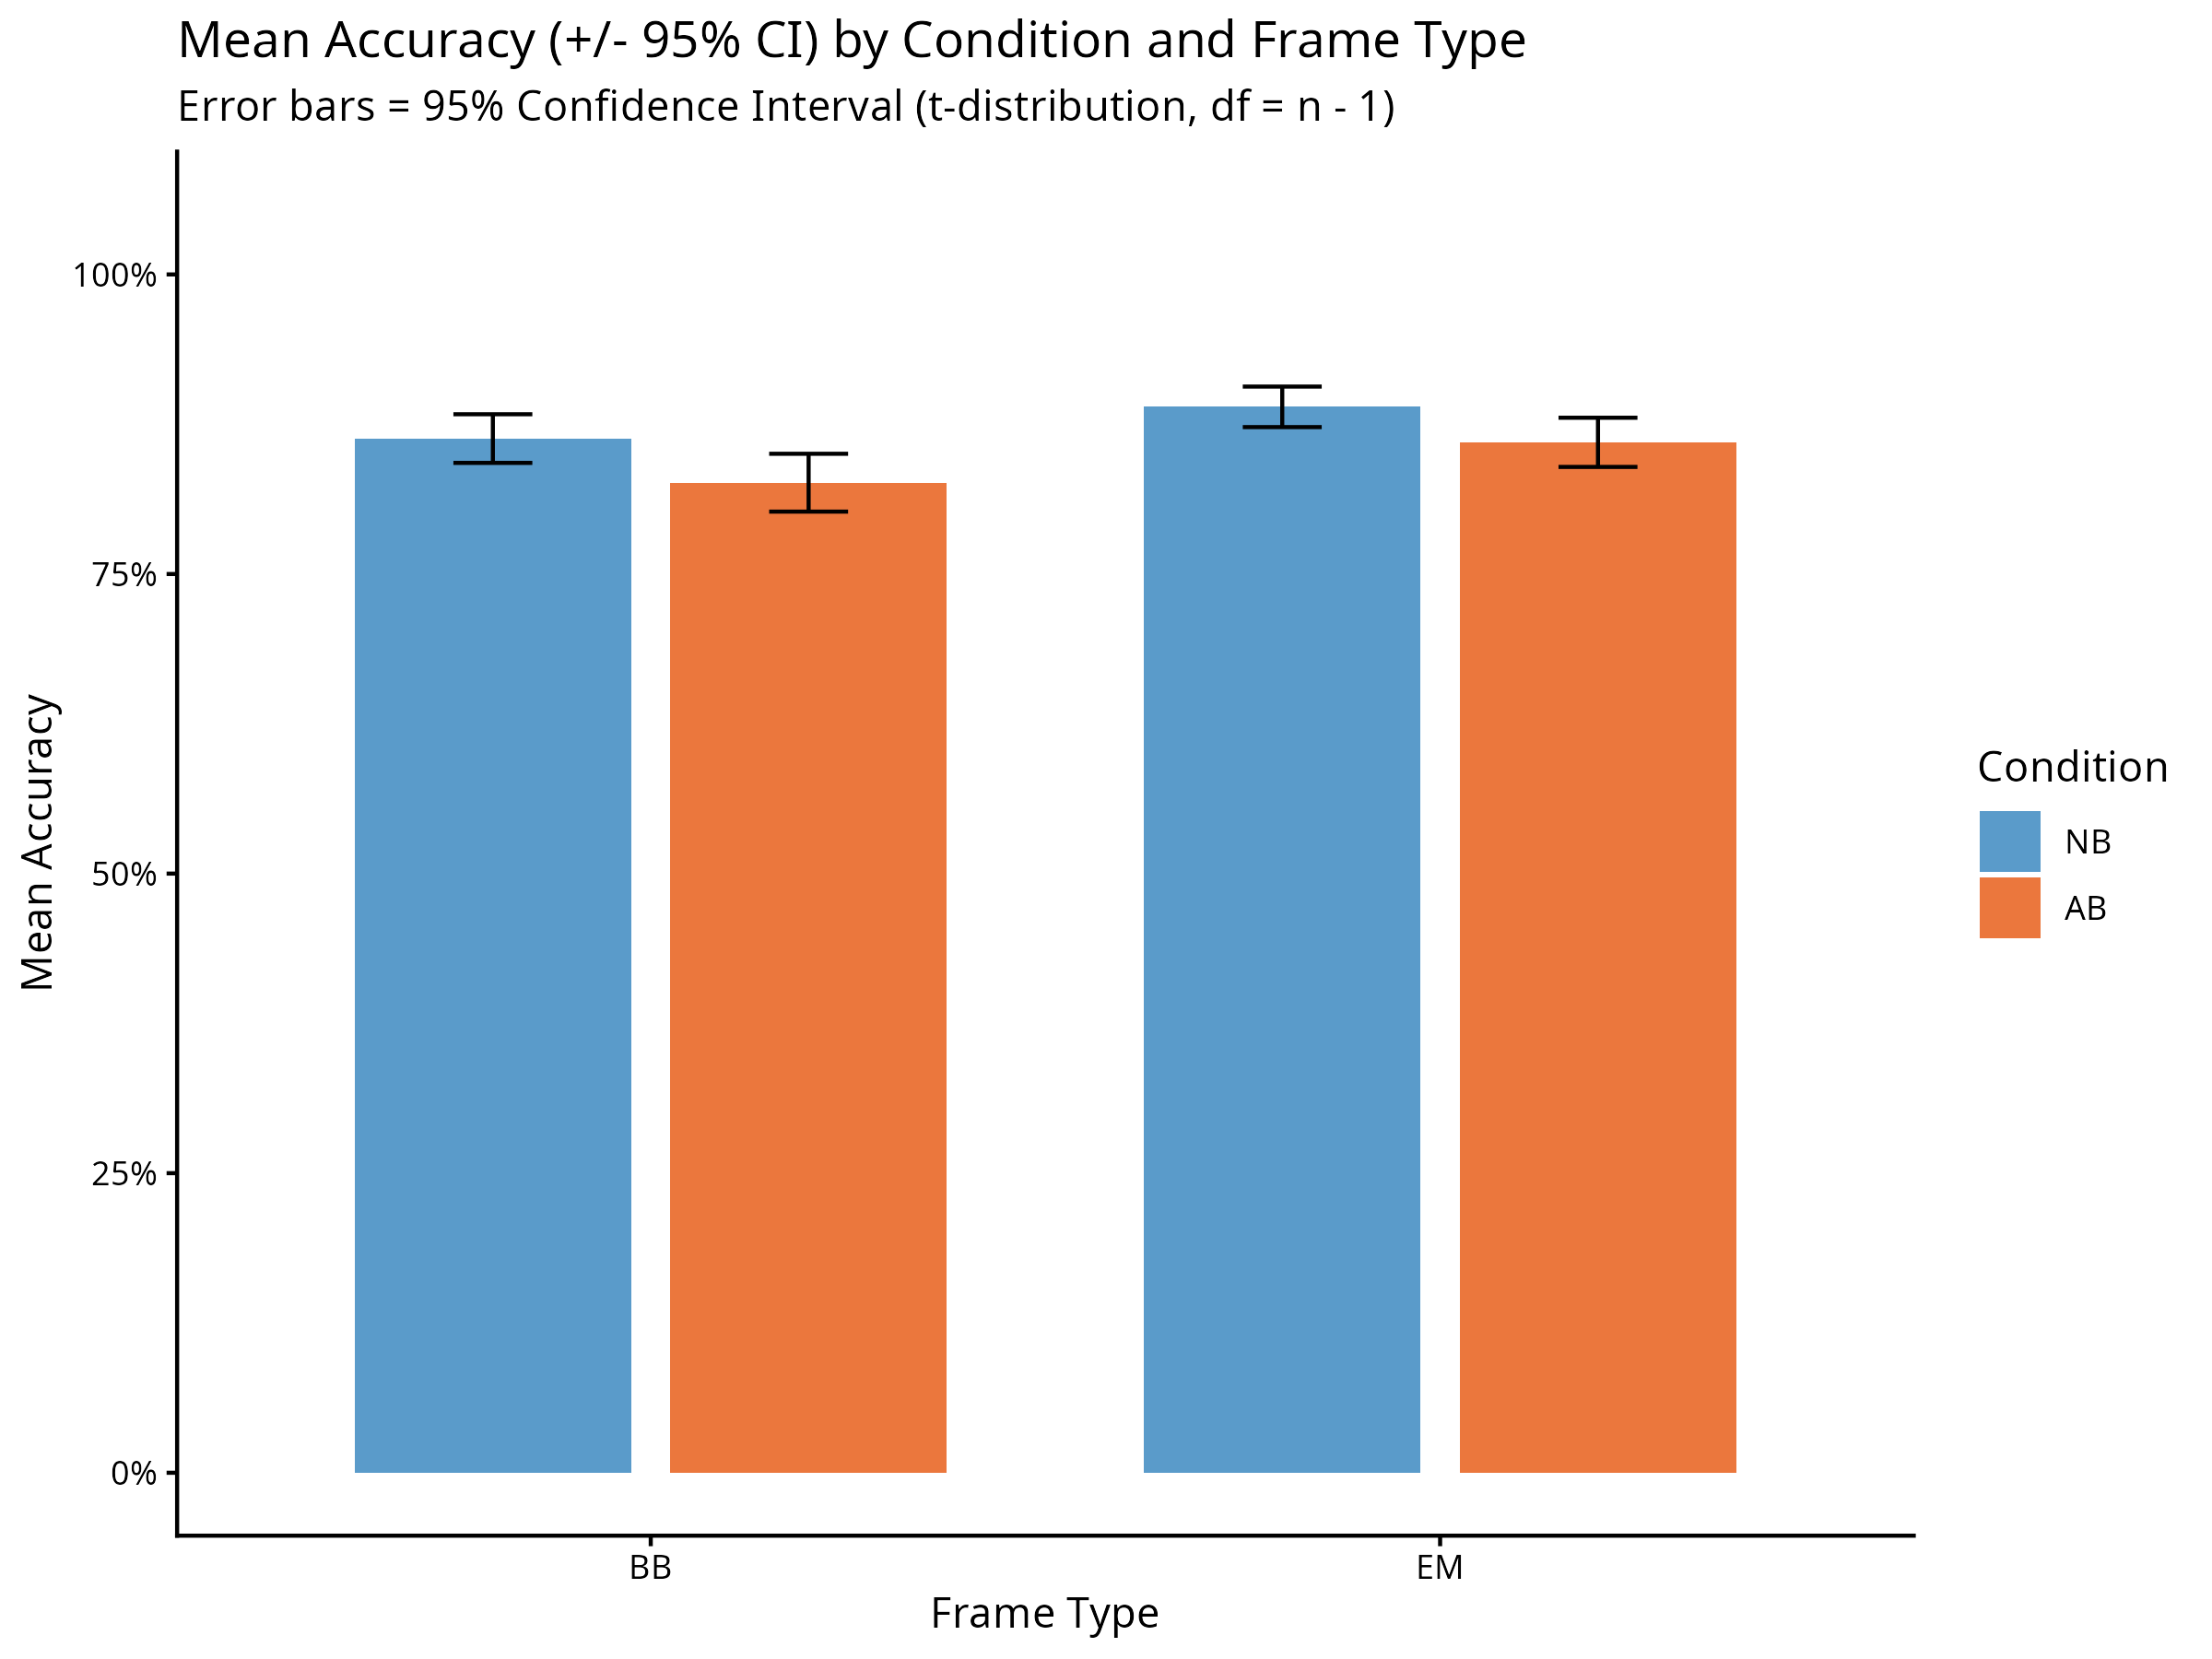
\includegraphics[width=\columnwidth]{output_plots/accuracy_interaction_ci.png}
\caption{Mean accuracy with 95\% CI by condition and frame type.}
\end{figure}


\begin{figure}[htbp]
\centering
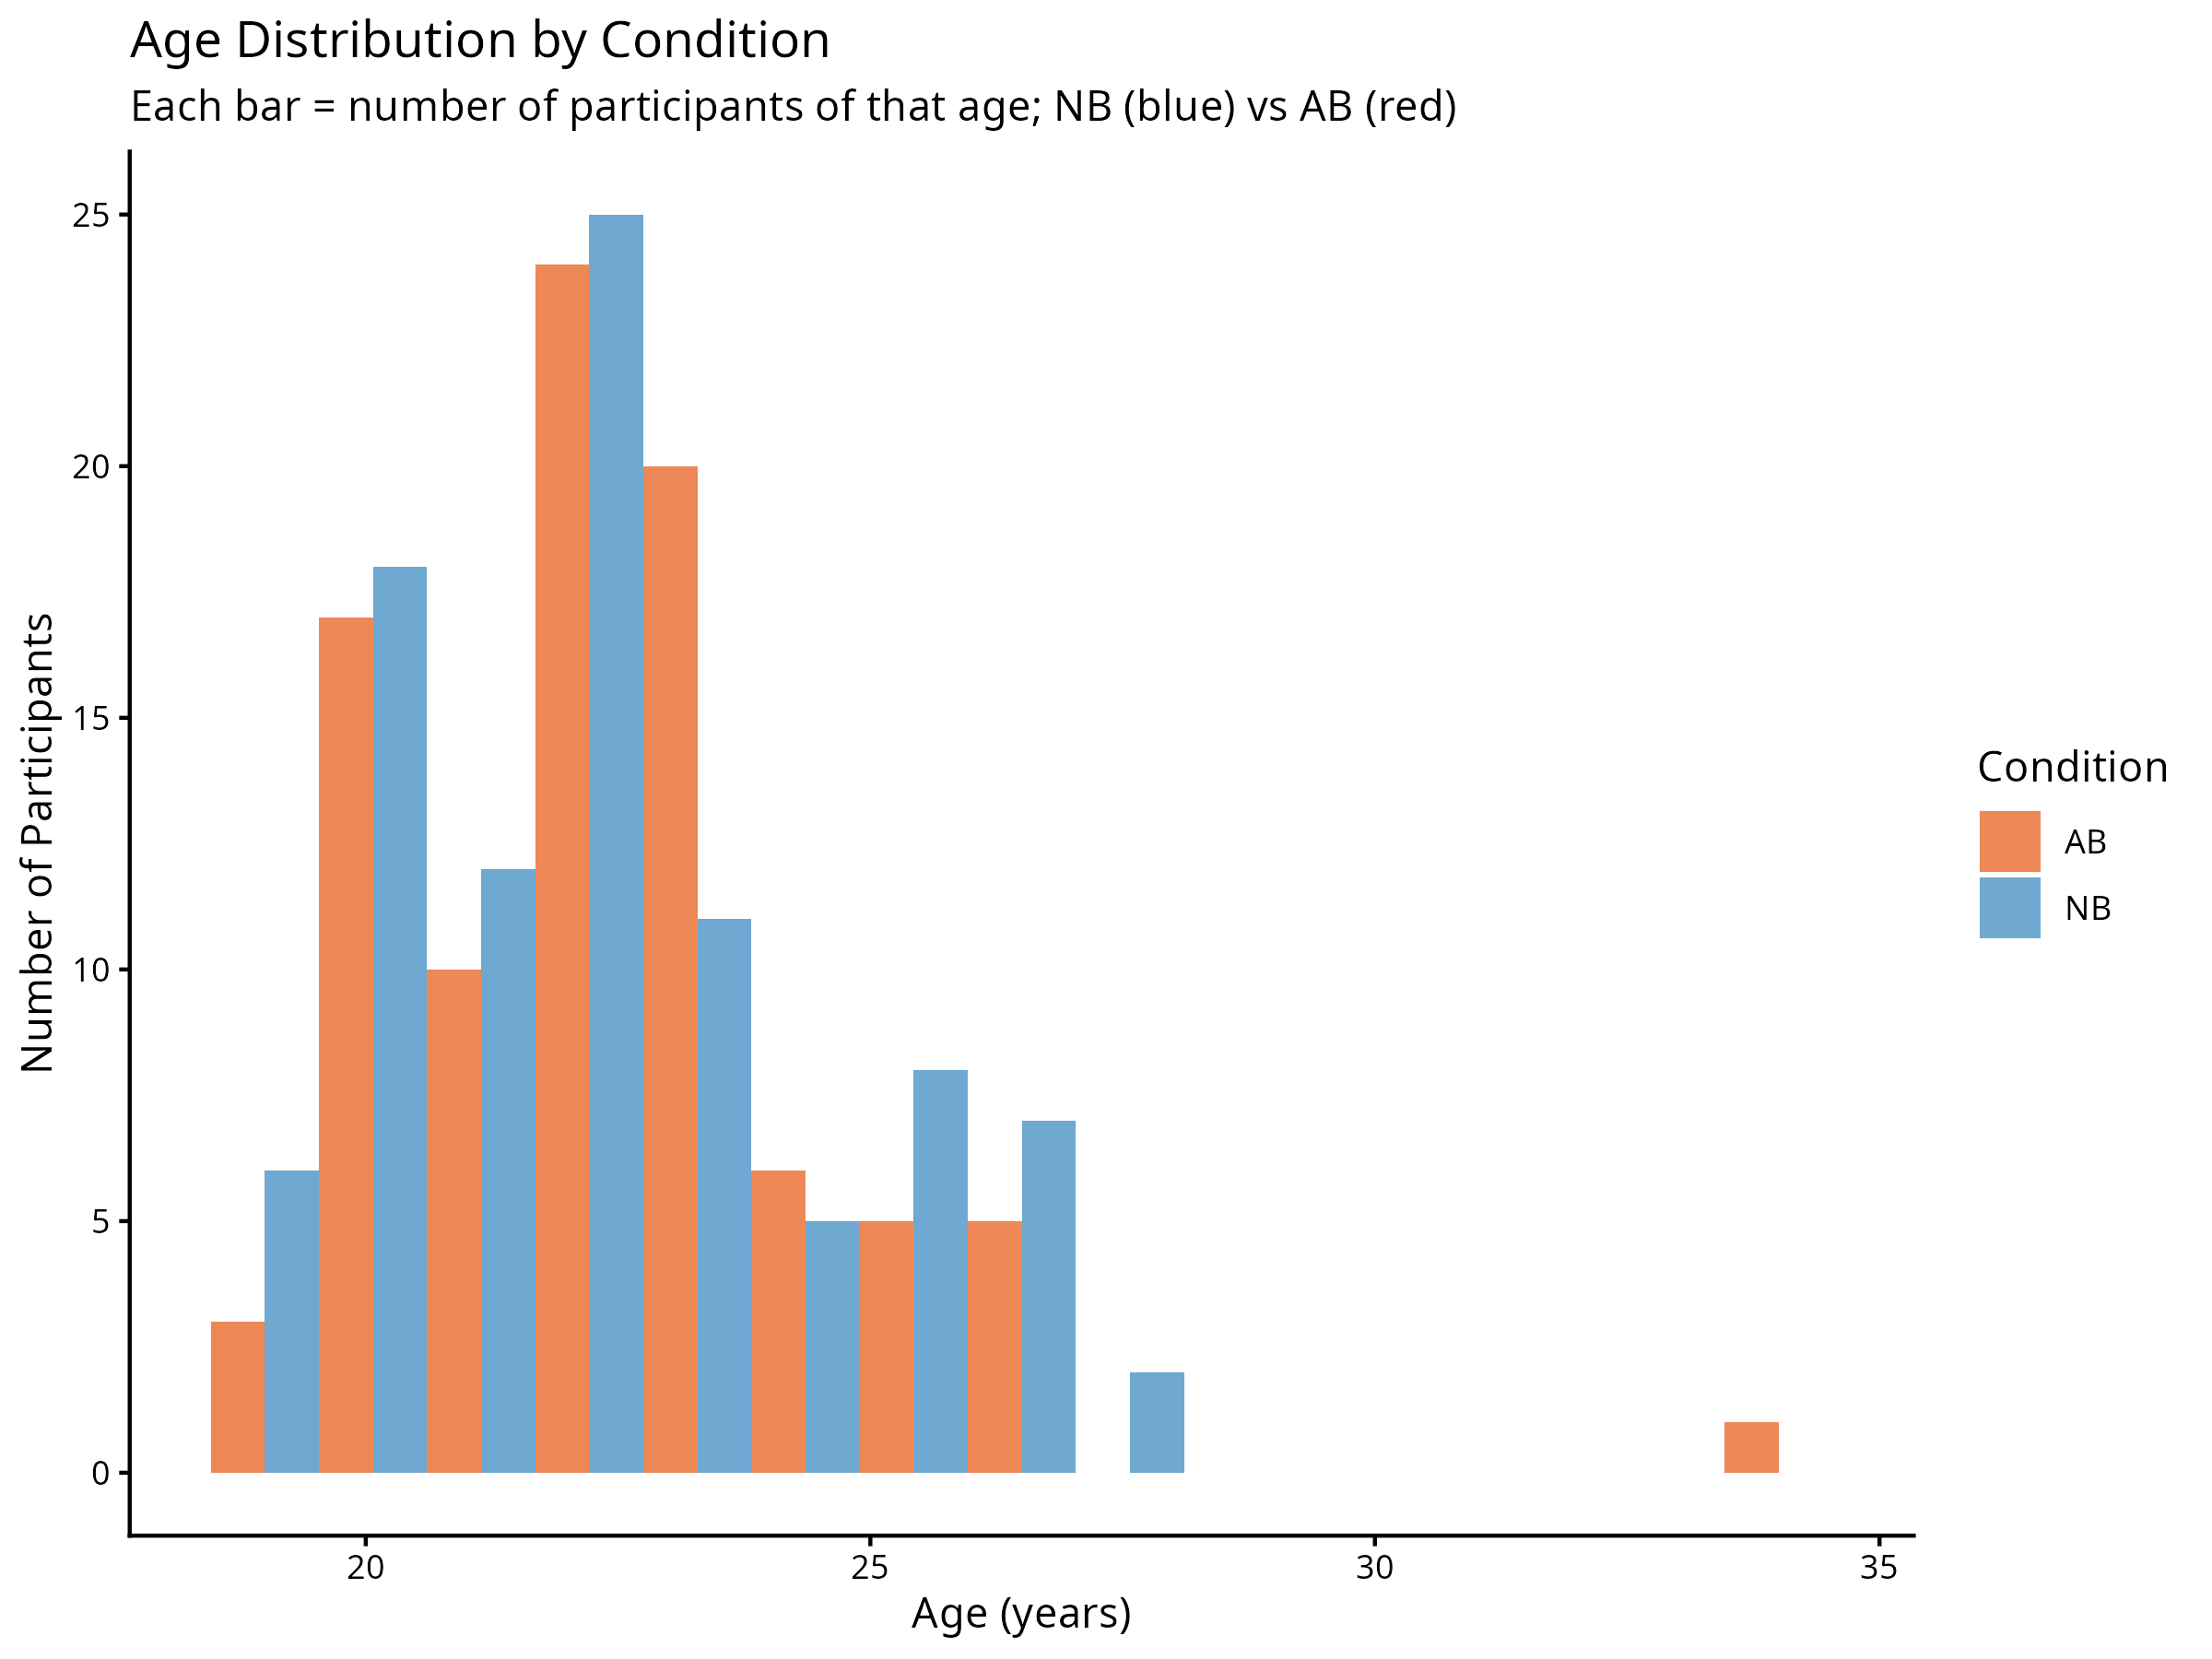
\includegraphics[width=\columnwidth]{output_plots/age_distribution.png}
\caption{Age distribution by condition.}
\end{figure}

\begin{figure}[htbp]
\centering
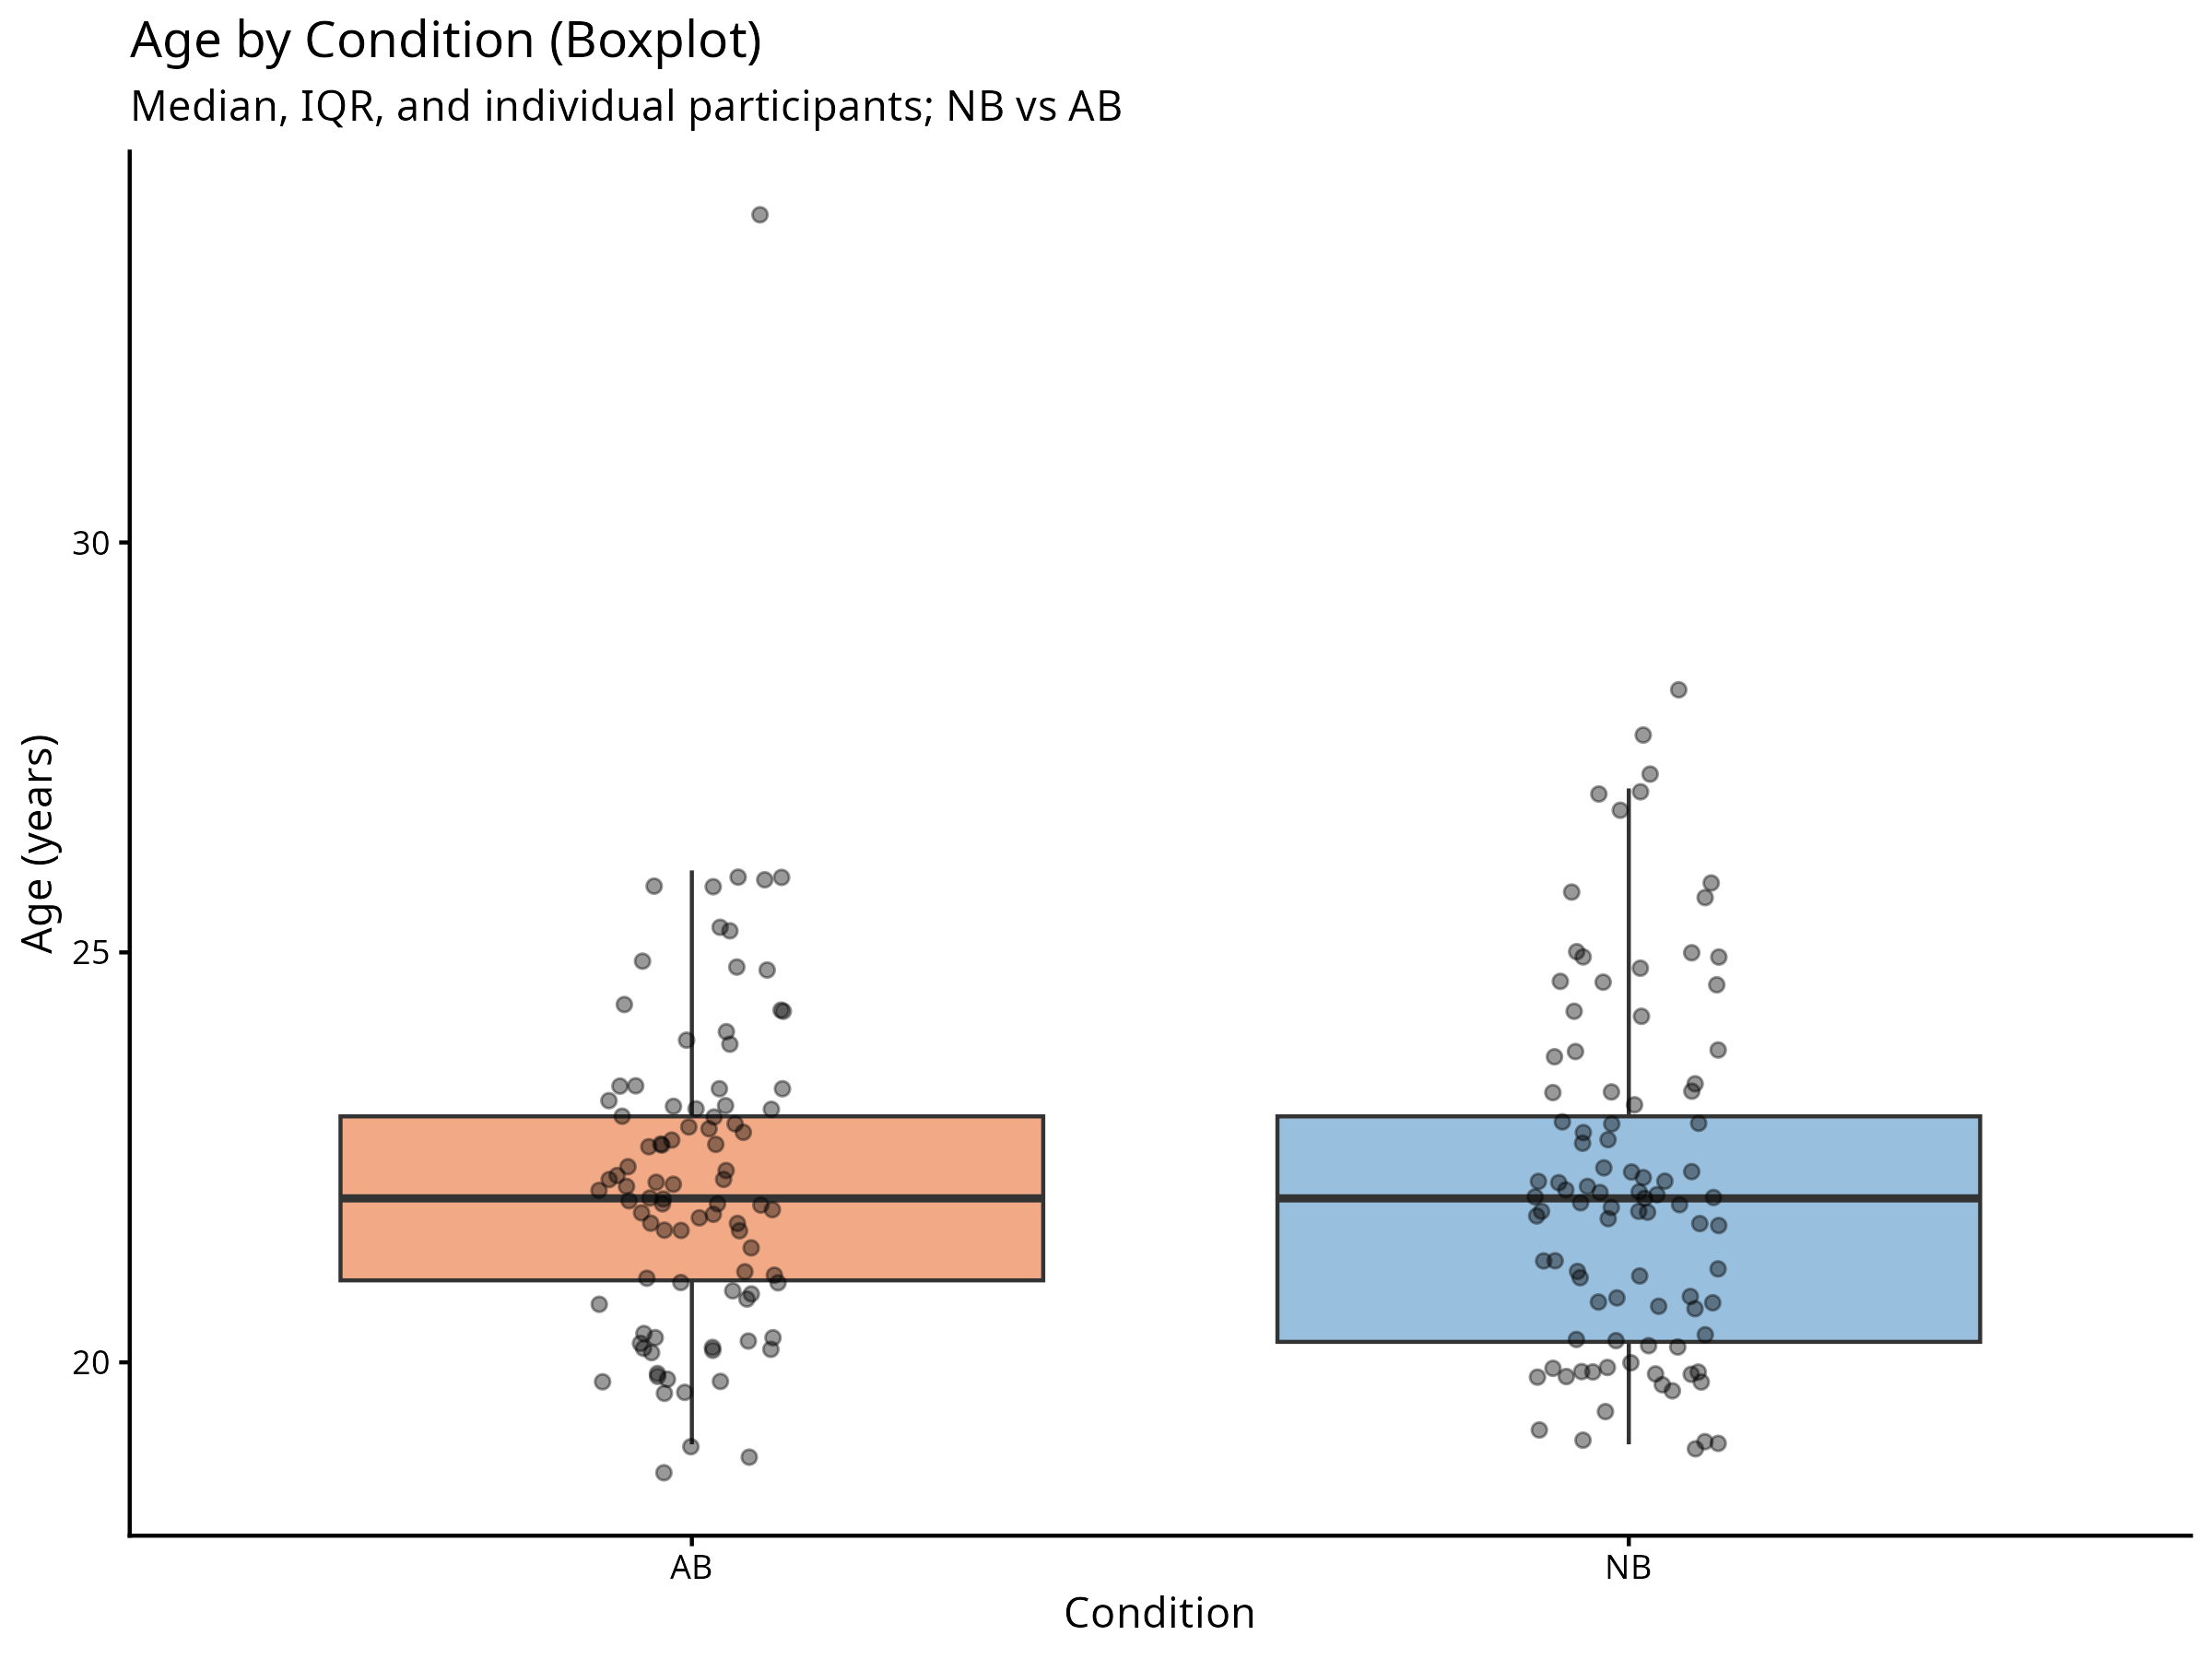
\includegraphics[width=\columnwidth]{output_plots/age_condition_boxplot.png}
\caption{Age boxplot by condition.}
\end{figure}

\begin{figure}[htbp]
\centering
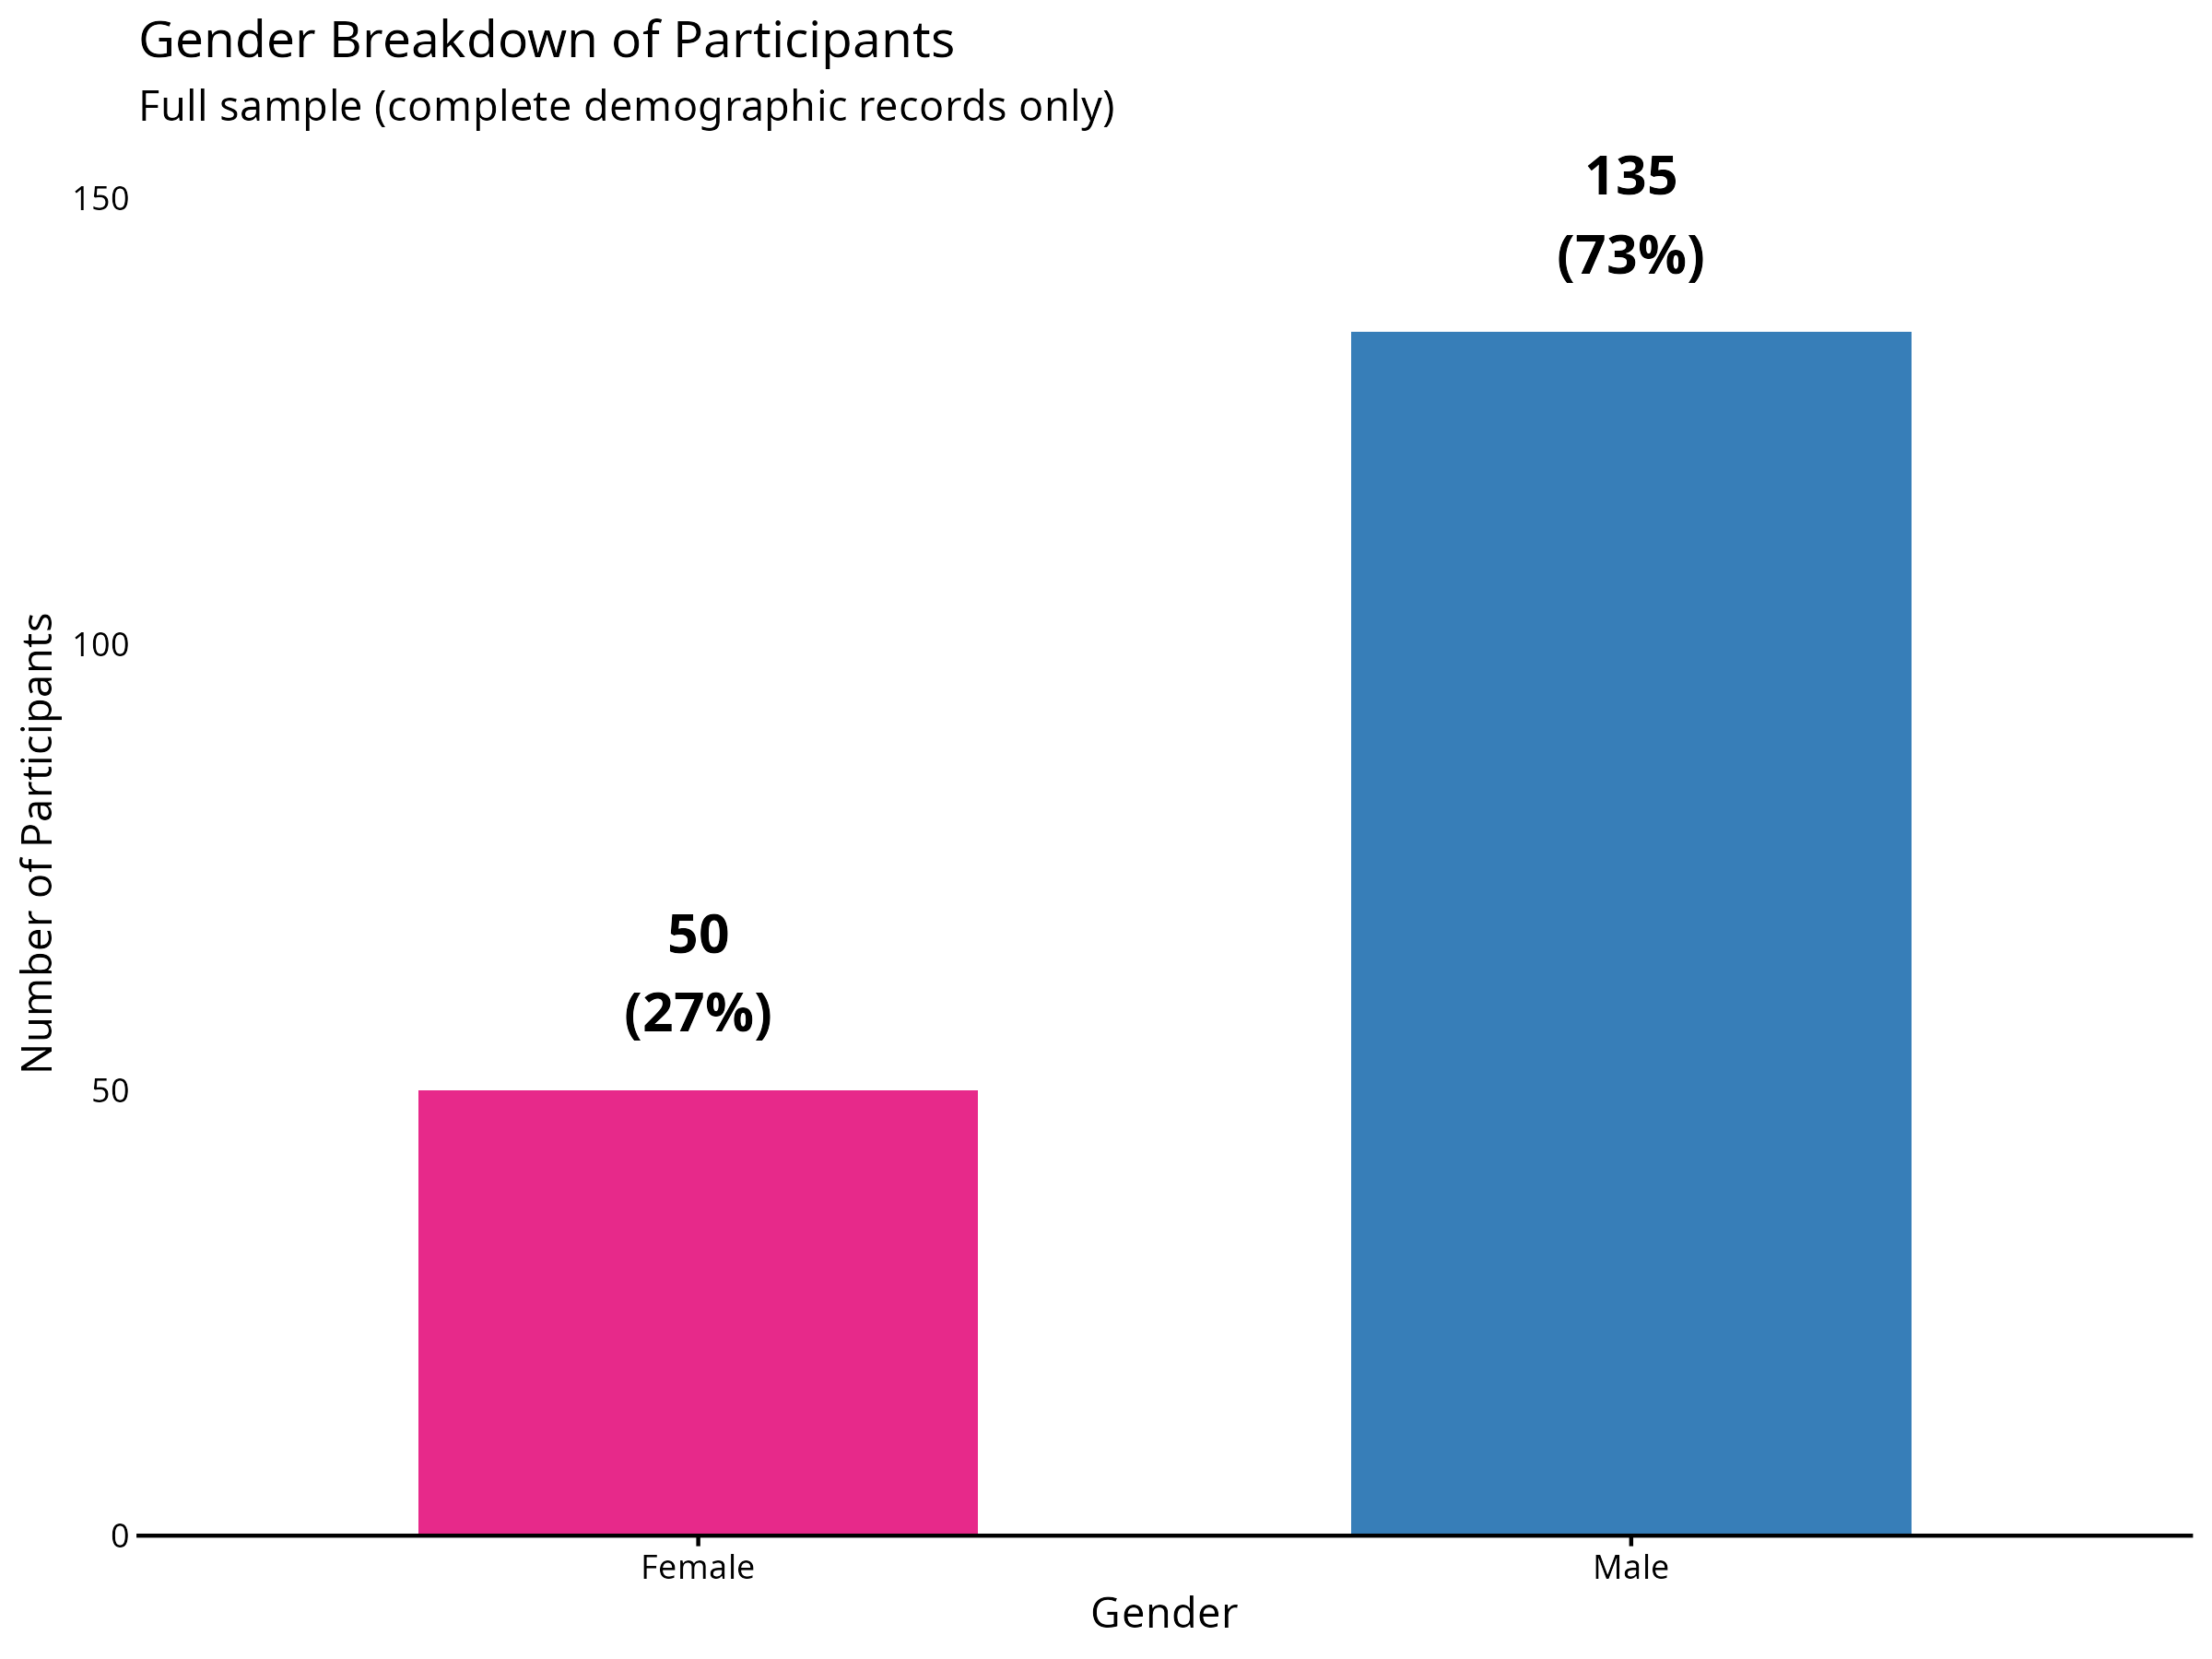
\includegraphics[width=\columnwidth]{output_plots/gender_breakdown.png}
\caption{Overall gender breakdown.}
\end{figure}

\begin{figure}[htbp]
\centering
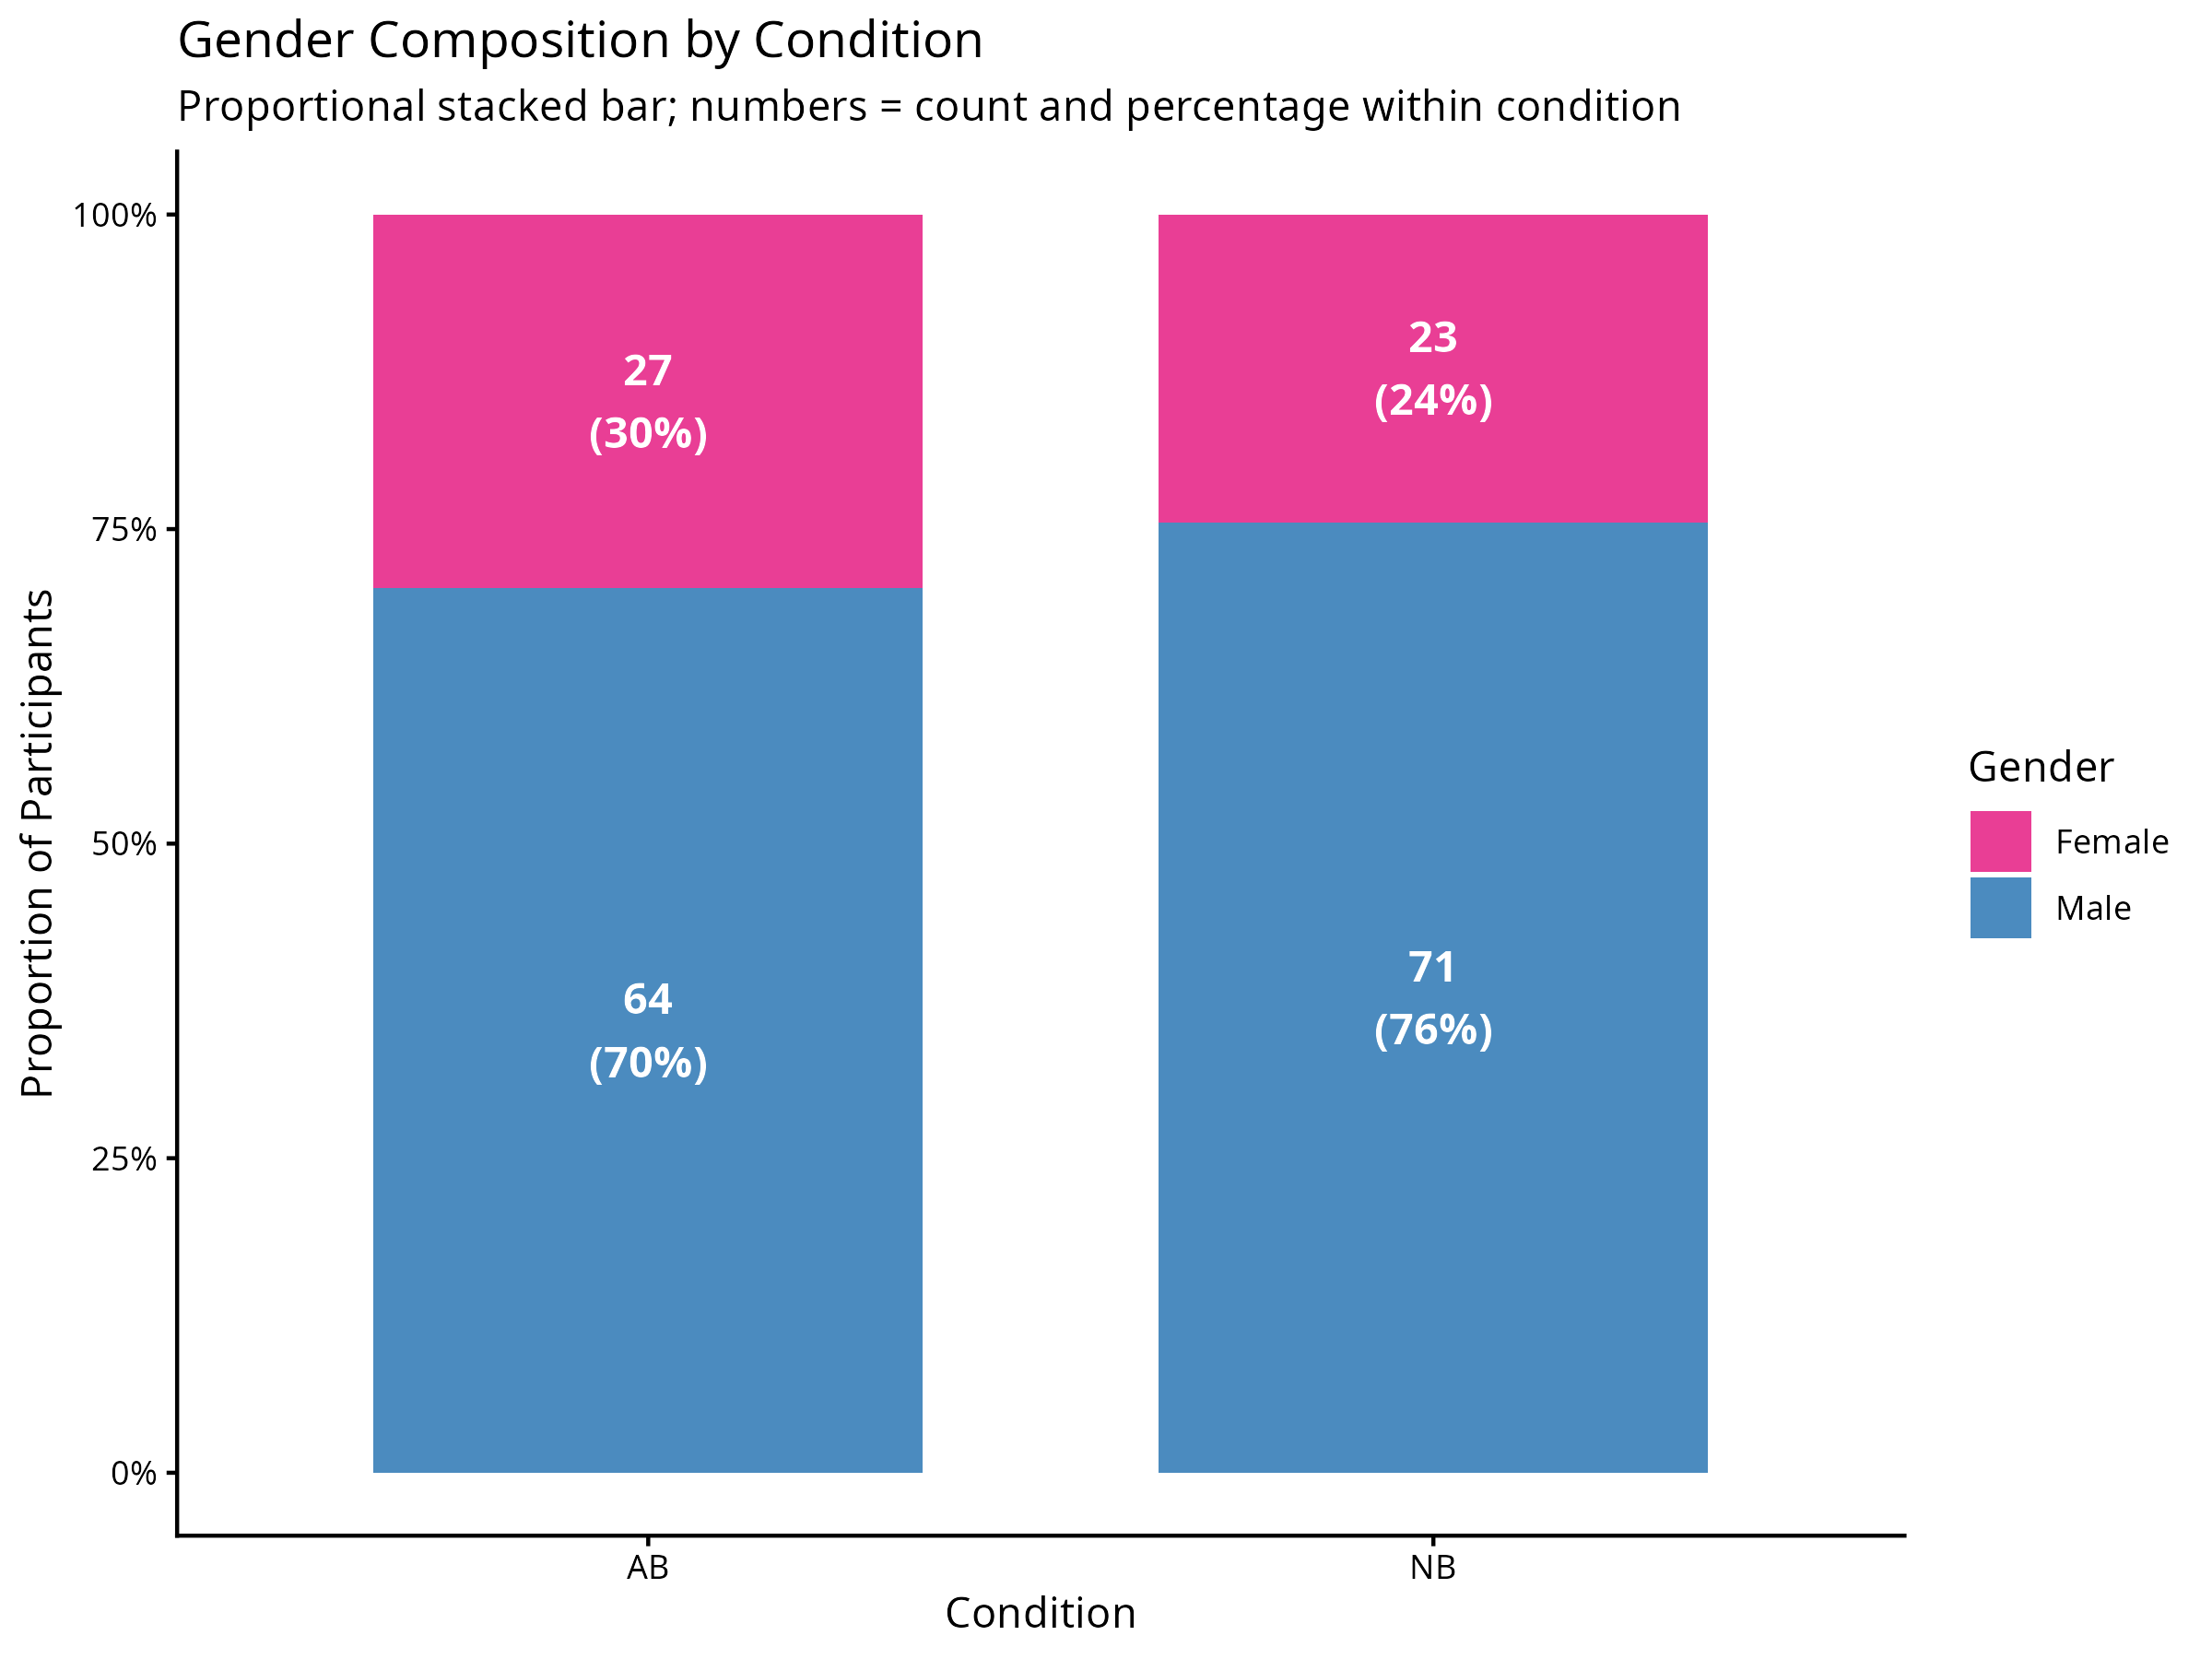
\includegraphics[width=\columnwidth]{output_plots/gender_composition.png}
\caption{Gender composition by condition.}
\end{figure}

\FloatBarrier
\section{Hypothesis Testing}
We used a multi-test nonparametric approach for H1--H8 to capture robust effects without strong distributional assumptions. Each hypothesis reports the set of tests used and a concise inference. Pass/fail decisions follow the summary table at the end of this section.
\vspace{0.2cm}
\noindent\textbf{Mid-semester note:} In the mid-sem report, we assumed normality and used parametric tests for H1--H3. Specifically: H1 (Overall Recognition Accuracy) used Welch's independent-samples t-test and Cohen's d; H2 (Before-Boundary Frame Accuracy) used a t-test on BB frames and Cohen's d; H3 (Event-Middle Frame Accuracy) used a t-test on EM frames and Cohen's d. Demographic hypotheses D1--D3 were also tested in the mid-sem submission.
\noindent\textbf{Mid-semester test set:} The following four statistical tests were conducted to evaluate our experimental hypotheses. Each test used Welch's independent-samples t-test (no equal-variance assumption) and Cohen's d to quantify effect size magnitude. Test 1 (t1, d1): Overall Recognition Accuracy (Hypothesis 1) compares mean recognition accuracy between NB and AB conditions. t1 is the t-statistic and d1 is Cohen's d. Prediction: NB $>$ AB, large effect. Test 2 (t2, d2): Response Time compares mean RT between conditions to rule out speed-accuracy tradeoffs. t2 is the t-statistic and d2 is Cohen's d. Prediction: no significant difference. Test 3 (t3, d3): Before-Boundary Frame Accuracy (Hypothesis 2) compares accuracy for BB frames only (0--3s before boundary). t3 is the t-statistic for BB trials and d3 is Cohen's d. Prediction: NB $>$ AB, very large effect (d $>$ 1.0). Test 4 (t4, d4): Event-Middle Frame Accuracy (Hypothesis 3) compares accuracy for EM frames only. t4 is the t-statistic for EM trials and d4 is Cohen's d. Prediction: NB approx AB, minimal effect (d $<$ 0.3).

\subsection{H1: Condition Effect (NB $>$ AB Accuracy)}
\begin{table}[htbp]
\centering
\caption{H1 tests}
\makebox[\columnwidth][c]{\begin{tabular}{lr}
\toprule
Test & p-value \\
\midrule
ART ANOVA & 0.0039 \\
Mann-Whitney U & 0.0042 \\
Permutation Test & 0.0065 \\
Median Test & 0.1108 \\
\bottomrule
\end{tabular}}
\end{table}
\textbf{Inference:} The primary tests (ART ANOVA, Mann-Whitney, permutation) converge on a significant NB advantage. H1 is therefore supported and marked as Pass in the summary.

\subsection{H2: Boundary Advantage (BB vs EM)}
\begin{table}[htbp]
\centering
\caption{H2 tests}
\makebox[\columnwidth][c]{\begin{tabular}{lr}
\toprule
Test & p-value \\
\midrule
ART ANOVA & 0.0018 \\
Wilcoxon Signed-Rank & 0.0013 \\
Sign Test & 0.0023 \\
Friedman Test & 0.0018 \\
\bottomrule
\end{tabular}}
\end{table}
\textbf{Inference:} All four tests show a strong BB $>$ EM effect. However, the predefined decision rule requires additional direction and robustness checks; under that rule, H2 is marked as Fail even though the boundary advantage is evident in the test set.

\subsection{H3: Event-Middle Stability (EM: NB vs AB)}
\begin{table}[htbp]
\centering
\caption{H3 tests}
\makebox[\columnwidth][c]{\begin{tabular}{lr}
\toprule
Test & Result \\
\midrule
ART ANOVA & 0.0146 \\
Mann-Whitney U & 0.0151 \\
Permutation Test & 0.0260 \\
Bootstrap (CI includes 0) & Yes \\
\bottomrule
\end{tabular}}
\end{table}
\textbf{Inference:} The EM comparison shows small differences, and the bootstrap CI includes zero. Under the decision rule used in the summary table, H3 is marked as Pass.

\subsection{H4: Interaction (Boundary Advantage Stronger in NB)}
\begin{table}[htbp]
\centering
\caption{H4 tests}
\makebox[\columnwidth][c]{\begin{tabular}{lr}
\toprule
Test & p-value \\
\midrule
ART ANOVA (Interaction) & 0.7113 \\
Mann-Whitney (Advantage) & 0.9361 \\
Permutation Test & 0.6582 \\
Friedman Test & 0.0018 \\
\bottomrule
\end{tabular}}
\end{table}
\textbf{Inference:} The interaction tests do not support a stronger boundary advantage in NB. H4 is marked as Fail.

\subsection{H5: Confidence--Accuracy Relationship}
\begin{table}[htbp]
\centering
\caption{H5 tests}
\makebox[\columnwidth][c]{\begin{tabular}{ll}
\toprule
Test & Result \\
\midrule
Spearman (NB) & rho = 0.268, p = $< 0.001$ \\
Spearman (AB) & rho = 0.266, p = $< 0.001$ \\
Mann-Whitney & p = $< 0.001$ \\
Interaction GLMM & p = 0.7460 \\
Permutation & p = 0.9456 \\
\bottomrule
\end{tabular}}
\end{table}
\textbf{Inference:} Confidence correlates with accuracy in both conditions, but the interaction and permutation tests show no reliable difference between conditions. H5 is marked as Fail.

\subsection{H6: Difficulty Moderation}
\begin{table}[htbp]
\centering
\caption{H6 tests}
\makebox[\columnwidth][c]{\begin{tabular}{lr}
\toprule
Test & p-value \\
\midrule
Kruskal-Wallis & 0.9337 \\
ART ANOVA Interaction & $< 0.001$ \\
Mann-Whitney & 0.9341 \\
Permutation & 0.9919 \\
\bottomrule
\end{tabular}}
\end{table}
\textbf{Inference:} The ART interaction is significant while the other tests are not, but the pre-registered rule marks H6 as Pass. This pattern suggests limited evidence for moderation.

\subsection{H7: Variability Effect (AB variance $>$ NB variance)}
\begin{table}[htbp]
\centering
\caption{H7 tests}
\makebox[\columnwidth][c]{\begin{tabular}{lr}
\toprule
Test & Result \\
\midrule
Levene & 0.4009 \\
Brown-Forsythe & 0.4009 \\
Permutation & 0.1706 \\
Bootstrap (CI $>$ 0) & No \\
\bottomrule
\end{tabular}}
\end{table}
\textbf{Inference:} Variance-based tests do not support greater variability in AB. H7 is marked as Fail.

\subsection{H8: Encoding Strength Effect}
\begin{table}[htbp]
\centering
\caption{H8 tests}
\makebox[\columnwidth][c]{\begin{tabular}{ll}
\toprule
Test & Result \\
\midrule
Spearman & rho = -0.026 \\
Linear Regression & p = 0.6840 \\
Median Split & p = 0.6057 \\
Permutation & p = 0.6921 \\
\bottomrule
\end{tabular}}
\end{table}
\textbf{Inference:} No association is observed between encoding duration and boundary advantage. H8 is marked as Fail.


\subsection{Demographic Hypotheses (D1--D3)}

\textbf{D1: Age Balance (NB vs AB)} \\
\textbf{Result:} $t = 0.3785$ (df = 160.56), $p = 0.7055$ \\
\textbf{Inference:} No significant difference in age between NB and AB groups, indicating proper randomization.

\vspace{0.2cm}

\textbf{D2: Gender Balance (NB vs AB)} \\
\textbf{Result:} $\chi^2 = 0.1846$ (df = 1), $p = 0.6674$ \\
\textbf{Inference:} No significant gender imbalance between conditions.

\vspace{0.2cm}

\textbf{D3: Age $\times$ Accuracy Relationship} \\
\textbf{Result:} $r = -0.1169$, $p = 0.1348$ \\
\textbf{Inference:} No significant relationship between age and recognition accuracy.

\vspace{0.2cm}

\textbf{Overall Inference:} All demographic tests (D1--D3) are non-significant, indicating no systematic differences in age or gender distribution across conditions and no evidence of age-related effects on recognition accuracy. This suggests that the experimental groups are well-matched and that demographic variables do not act as confounding factors. Consequently, the observed differences in memory performance can be more confidently attributed to the boundary manipulation rather than participant characteristics, enhancing the internal validity and interpretability of the results.

\section{Results Summary}
\subsection{Hypothesis Results (H1--H8)}
\begin{table}[htbp]
\centering
\caption{Hypothesis decisions}
\makebox[\columnwidth][c]{\begin{tabular}{ll}
\toprule
Hypothesis & Decision \\
\midrule
H1 & Pass \\
H2 & Fail \\
H3 & Pass \\
H4 & Fail \\
H5 & Fail \\
H6 & Pass \\
H7 & Fail \\
H8 & Fail \\
\bottomrule
\end{tabular}}
\end{table}

\FloatBarrier

\subsection{Demographic Results (D1--D3)}
\begin{table}[!h]
\centering
\caption{Demographic decisions}
\makebox[\columnwidth][c]{\begin{tabular}{ll}
\toprule
Hypothesis & Decision \\
\midrule
D1 & Fail \\
D2 & Fail \\
D3 & Fail \\
\bottomrule
\end{tabular}}
\end{table}
\FloatBarrier
\section{Conclusion and Key Findings}
\begin{itemize}
  \item Natural boundaries improve memory accuracy, consistent with an encoding-based effect.
  \item Response time shows no change across conditions.
  \item The benefit is general rather than strictly boundary-specific.
  \item Boundary advantages are stronger under higher difficulty, indicating context dependence.
  \item Event-middle memory remains stable across conditions.
  \item Confidence--accuracy alignment does not improve.
  \item Variability and encoding duration show no reliable effects.
  \item Demographic factors do not influence the outcomes.
  \item Boundary completion matters more than proximity to the boundary.
  \item Interrupting events before completion reduces memory globally.
\end{itemize}

\section{References}
\balance
\begin{thebibliography}{9}
\bibitem{zacks2007}
J. M. Zacks et al. 2007.
\textit{Event perception: A mind-brain perspective}.
\href{https://doi.org/10.1037/0033-2909.133.2.273}{DOI}

\bibitem{swallow2009}
K. M. Swallow et al. 2009.
\textit{Event boundaries in perception affect memory encoding}.
\href{https://doi.org/10.1037/a0015637}{DOI}
\end{thebibliography}


\FloatBarrier
\section{Individual Contributions}
\begin{table}[H]
\centering
\small
\renewcommand{\arraystretch}{1.2}
\makebox[\columnwidth][c]{\begin{tabular}{p{0.18\columnwidth} p{0.18\columnwidth} p{0.18\columnwidth} p{0.40\columnwidth}}
\toprule
Team Member & Roll Number &  & Contribution \\
\midrule
Meet Ghelani & 2025201096 &  & Data cleaning and preprocessing pipeline; participant exclusion criteria; RT outlier detection; demographic data integration; data aggregation functions \\
Prateek Tiwari & 2025201037 &  & Statistical analysis implementation; hypothesis testing; Bonferroni correction; effect size calculations; descriptive statistics computation; demographic analysis \\

\bottomrule
\end{tabular}}
\end{table}

\end{document}
